\documentclass[main.tex]{subfiles}
\begin{document}
\glsresetall

\section{Introduction}

The \gls{lmc} is one of the closest satellite galaxies of the \gls{mw}, at a distance of $\sim$ 50 kpc \cite{2013LMCdistance1}. Thanks to its proximity, large volume and orientation angle ($\sim$ 30º \cite{2004StructureandOrientationLMC}), it is observed as an extended object of about 10º diameter in the sky, which has allowed the study of its structure and individual components in great detail. Observations of the \gls{lmc} in the whole electromagnetic spectrum have revealed the presence of a big number of extreme objects such as pulsars \cite{2013RadioPulsarsLMC} \cite{2016LMCFermiLAT}, \glspl{snr} \cite{2015MultiwavelengthLMCsnr} \cite{2012XMM1987} \cite{2016SNRinXrayLMC},  \gls{pwne} \cite{2015HESSTeVLMC} \cite{2016LMCFermiLAT} \cite{2003PWNeintheLMC} \cite{2008PWNeXrayLMC} and gamma-ray binaries \cite{2017HESSLMCP3}. Many of these objects are known to be cosmic-ray accelerators and therefore potential $\gamma$-ray emitters. $\gamma$-ray emission up to TeV energies from several sources within the \gls{lmc} has already been detected by the current generation gamma-ray experiments \textit{Fermi}-LAT and \gls{hess} and it is expected that many more objects will be discovered by the future \gls{cta}.\\
The remarkable interest of the \gls{lmc} for $\gamma$-ray astrophysics relies on its high star formation activity, which implies a high supernova rate and thus a large population of $\gamma$-ray sources. Also, it offers a unique opportunity to study the relation between star formation and cosmic-ray production and propagation, as an alternative to the \gls{mw}.\\
\glspl{cr} are an important component of \gls{ism} in galaxies, with energy densities comparable to that of magnetic fields. The origin and propagation of \glspl{cr} is still a field of study as well as their role in galaxy evolution. It is very likely that they have a significant effect in star formation, acting as an extrinsic feedback source. The basic idea is that, even the energy injection rate of \glspl{cr} is negligible compared to other by-products of star formation, such as photons, winds and supernova shocks, they interact with the \gls{ism} and exchange a significant amount of momentum. Studies on starburst galaxies luminosities \cite{2008SocratesCRandSF} have established that it is possible that cosmic-ray winds are produced in high star formation rate regions, perturbing the hydrostatic balance and truncating star formation. On the other hand, infrarred observations of \gls{ulrigs} suggest that \glspl{cr} are able to heat gas in molecular clouds and are their main agent of temperature regulation and ionization, fundamentally altering the initial conditions for star formation \cite{2010PapadopoulosCRinSF}.\\
While \gls{lmc} evolution is closely related to the \gls{mw} and the rest of the local group, the observations of very young globular clusters in the \gls{lmc} suggests that its \gls{sfh} is fundamentally different to that of the \gls{mw}. In fact, the \gls{lmc} is currently in a star formation epoch with a rate of $\sim$ 0.2 $M_{\odot}$ which was reignited 4-5 Gyrs ago after a dramatic event affecting the \gls{ms} (composed by the \gls{lmc} and the \gls{smc}) \cite{2009SFHofLMC}. The \gls{lmc} is classified as an irregular galaxy, the most common type in the universe. In general, irregular galaxies are simpler, less dusty and with lower metallicity than spiral galaxies (like the \gls{mw}). Because they are less evolved, they present higher gas content and lower abundance of heavy elements \cite{2013InfrarredLMC}. All these differences with respect to the \gls{mw} affecting the characteristics of the \gls{ism}, are fundamental for the study of the production and propagation of \glspl{cr} in star forming regions, and allow to use the \gls{lmc} as an alternative probe to the \gls{mw}.
Characterizing the \glspl{cr} origin and propagation throughout the \gls{ism} is not an easy task, as charged particles are deflected by magnetic fields, making it impossible to reconstruct their trajectories and thus, pointing back to their origin form Earth. The best way to study cosmic-ray physics in the galaxies is through the diffuse emission from radio to $\gamma$-rays that they produce when interacting with other particles in the \gls{ism} and the radiation of magnetic fields. The leptonic component of this emission, produced by cosmic-ray electrons, can be probed by radio, X-ray and $\gamma$-ray observations. The radio diffuse emission come from synchrotron emission of cosmic-ray electrons injected by supernova remnants. They can also suffer \gls{ic} scattering with photons of the interstellar radiation field or the cosmic microwave background, producing emission from X-ray to $\gamma$-rays \cite{2008ICgammaray}. The hadronic component of diffuse cosmic-ray emission is produced (mainly) by cosmic-ray proton inelastic collisions with the \gls{ism} particles, which produce pions resulting in a continuum $\gamma$-ray emission coming from pion decay \cite{1963Pimesonsproducegammarays}. As hadrons make up the 90\% of the \glspl{cr} composition, $\gamma$-rays are a fundamental probe for cosmic-ray production and propagation. 
A galaxy like the \gls{lmc}, externally viewed and nearly face on offers an unique opportunity for studying the diffuse distribution of \glspl{cr} in a galaxy, in comparison with the \gls{mw} which has the problem of line-of-sight confusion of sources. \textit{Fermi}-LAT observations of the \gls{lmc} revealed a diffuse $\gamma$-ray emission little correlated with the large scale distribution of the gas column density of the galaxy \cite{2010FermiLATLMC11months}. This correlation would be observed if cosmic-rays could freely diffuse in the \gls{ism} as it is observed in the \gls{mw}. Instead, it appears to be much more correlated with tracers of massive star forming regions such as the 30 Doradus region \cite{2012CRinLMC30Doradus}.\\
Beyond the extraordinary opportunities for cosmic-ray physics, the \gls{lmc} offers also the possibility to help solving the fundamental problem of \gls{dm}. The \gls{lmc} has a mass of the order of $10^9$ M$_{\odot}$ enclosed in 8.9 kpc and more than a half is due to a dark halo \cite{2002LMCkinematics}. Study of the rotational curves of the \gls{lmc} revealed that also it must contain a dark compact bulge with an anomalously high mass-to-luminosity ratio as large as $\sim 20-50$ \cite{1999LMCbulge} compared of that of the calculated for the \gls{mw} $\sim$ 7 M/L \cite{2013MWbulge}. With these characteristics, \gls{lmc} would be the most \gls{dm} massive object after the \gls{gc} offering an alternative source for indirect searches of \gls{dm} signal.\\
Among all the theories trying to explain the nature of \gls{dm}, the \gls{wimp} theory is one of the most popular, explaining \gls{dm} as a particle which can suffer annihilation or decay into \gls{dm} particles. Different channels of annihilation would produce a certain spectrum of gamma-rays \cite{2011cirelli} which could be detected as an excess over the $\gamma$-ray flux produced by baryonic backgrounds. Following this scheme, \textit{Fermi}-LAT used five years of data to search for a \gls{dm} annihilation signal in $\gamma$-rays and placed competitive bounds on the annihilation cross section as a function of the dark matter particle mass and annihilation channel \cite{2010FermiLATLMC11months}.\\
The \gls{lmc} Survey is one of the \gls{ksp} of \gls{cta} \cite{2019SciencewithCTA}, with more than 300h of dedicated observations and many scientific objectives: population studies of \glspl{snr} and \gls{pwne}, transport of \glspl{cr} and searches of \gls{dm}.
In this chapter, which is the core of this thesis, a characterization of the \gls{lmc} in the energy range of \gls{cta} is performed, in order to cast predictions on the possible results of the \gls{lmc} survey. Our methodology is to build an emission model of the \gls{lmc} and use a dedicated \gls{cta} software to perform simulations of the survey data products. We use a maximum likelihood approach to calculate the detection significance of the different sources of $\gamma$-rays in the \gls{lmc}, and to set a realistic model of the diffuse cosmic-ray emission. In the same way, we calculate sensitivity curves for the detection of a possible \gls{dm} annihilation signal.\\

As has already been mentioned, the \gls{lmc} has been observed by \textit{Fermi}-LAT and \gls{hess} in the \gls{he} and \gls{vhe} ranges. To perform predictions on how the \gls{lmc} will look like in the range of \gls{cta}, up to hundreds of TeV, we must rely on the previous observations and make assumptions on how the emission extrapolate to higher energies. The $\gamma$-ray emission in the \gls{lmc} can be divided in two types: emission from point-like sources and diffuse emission from \glspl{cr}. The idea is to build a complete emission model of the \gls{lmc} which afterwards will be convolved with \gls{cta} \glspl{irf} to simulate the data which will be obtained from the \gls{lmc} survey using the software \textit{ctools}, described in chapter \ref{cap:CTA}. These simulations are used to cast predictions on the detectability of the sources included in the emission model. These predictions include the calculation of the detection significance of the model components, a study on the sensitivity of \gls{cta} to the detection a point-source with a power law spectrum in the \gls{lmc}, a population study of detetable \gls{pwne} and the sutyd of the possible diffuse emission models detectable by \gls{cta}, focusing on its ability to differentiate between large and small scale emission.\\
The emission model computed is also used as background for the potential detection of a \gls{dm} annihilation signal. The results on this topic are given in the shape of sensitivity curves for the detection of an array of \gls{dm} models, characterized by density profile, annihilation spectrum and \gls{dm} particle mass.

\section{Emission Model} \label{sec:model}

In this section, the emission model developed for the global $\gamma$-ray emission of the \gls{lmc} is described. The baseline model consist on four already-known \gls{vhe} point-like sources, galaxy-scale insterstellar emission of both hadronic and leptonic origin, and a population of \gls{pwne}. 

\subsection{Diffuse emission} \label{sec:diffusemodel}
Interstellar diffuse emission of $\gamma$-rays in the \gls{lmc} is produced by the interaction of \gls{cr} with the \gls{ism}. Two kinds of interactions were considered to compute the diffuse emission model: \gls{ic} processes from \gls{cr} electrons and pion-decay from proton interactions. The distribution of \glspl{cr} in the \gls{lmc} has been computed under the assumptions of steady \gls{cr} injection from an ensemble of point sources, followed by diffusive transport in the \gls{ism} and interaction with simplified distributions for interstellar components (gas, photon and magnetic fields). The resulting interstellar emission model is obtained by convolving the distribution of injection sources with average emission kernels for pion-decay and \gls{ic} scattering, plus a correction by the actual gas distribution for the pion-decay.\\
As has been discussed in chapter \ref{cap:gammarayastro}, \glspl{cr} are accelerated by the power provided by winds and outflows around massive stars, supernova explosions and compact objects. Star forming regions (H II regions) serve as tracers for this kind of objects. The HII regions catalog from \cite{2012HIIinLMC} was used as template for the distribution of \gls{cr} sources, taking only regions with $H\alpha$ luminosy above $10^{37}$ erg s$^{-1}$, where the assumption of steady \gls{cr} injection is valid. The most luminous HII region in the \gls{lmc} is 30 Doradus, with a luminosity of $10^{39.66}$ erg s$^{-1}$. It is not included in the injection model because its mostly populated by very young OB stars (< 4 Myrs) \cite{201130Doradusstarforming} and is unlikely that many \gls{sne} have exploded recently in the region. The \gls{cr} injection power is assumed to be proportional to the ionizing luminosity of the HII regions. The total \gls{cr} injection power is assumed to be constant in time, corresponding to the release of $E_{SN} = 10^{51}$ erg per \gls{sn} explosion, at an estimated rate of $r_{SN} =  0.002$ SN yr$^{-1}$ \cite{1991SNrates}, where the fraction of mechanical energy trapped by \gls{cr} acceleration is $\eta_{p} = 10^{-1}$ for protons and $\eta_{e} = 10^{-3}$ for electrons. This total power is dsitributed among all the different star forming regions in proportion to their ionizing luminosity.
The injection spectra is assumed to follow a power-law distribution in momentum, with an spectral index for protons(electrons) of 2.45(2.65), starting at 1 GeV/c, with an exponential cut off at 1 PeV/s.\\
The diffusion of \gls{cr} away from their sources is assumed to occur due to spatial diffusion and energy losses. Energy loss processes include hadronic interations for \gls{cr} protons and synchroton, \gls{ic} scattering and Bremsstrahlung radiation for \gls{cr} electrons, interacting with the homogeneous gas, photons and magnetic fields of the \gls{ism} model adopted. The spatial distribution of protons and electrons around a stationary source is computing by integrating the solution of the diffusion loss equation, as of \cite{2006diffusionloss}, over an injection duration of $T_{inj} = 100$ Myr. This accounts for the star formation histori in the \gls{lmc} which was not steady over recent times and exhibits a drop in star formation at 100 Myr \cite{2009SFHofLMC}. Surface brightness angular profiles are computed by integrating the particle spatial distributions along the line of sight over a thickness 2H, where H is the half-thickness representative of the target distribution: a 180 pc gas disk scale height for \gls{cr} protons and a 1 kpc magnetic and radiation field halo for \gls{cr} electrons. The result of these calculations are the emission kernels for \gls{ic} and pion-decay, which was convolved with the \gls{cr} source distribution. Furthermore, for the pion-decay component a nuclear enahncement factor of 1.753 is introduced to account for the contribution of helium and heavier nuclei in \glspl{cr} and the \gls{ism}. Also, the resulting emission cube is rescaled by the gas column density map of the \gls{lmc}, to recover the actual gas distribution structure of the galaxy.\\
About the decription used for the \gls{ism} medium in the \gls{lmc}  an average \gls{ism} model has been computed, which includes a description of the interstellar conditions in terms of gas mass and structure, stellar population feeding the radiation fields and magnetic field configuration. The \glspl{cr} transport and subsequent $\gamma$-ray emission will be strongly affected by the characteristics of this \gls{ism}. For the interstellar gas, a disk having a radius of 3.5 kpc and a scale height of h=0.18 kpc has been used, where the mass of atomic, molecular and ionised hydrogen has been computed. The interstellar radiation field model has been developed following the work of \cite{2014DustEMLMCismemission}, where the broadband infrared dust emission in the \gls{lmc} is computed for typical HII regions. About the magnetic field, the total magnetic field strenght in the \gls{lmc} is calculated to be 4.3 $\mu$G \cite{2005LMCmagneticfield}.     


\subsection{Point Sources}\label{sec:point}

Observations in gamma-rays of the \gls{lmc} have provided a very interesting catalog of point-like sources of different nature, which have revealed very interesting features. For this work, we use the \gls{lmc} data collected by \textit{Fermi}-LAT \cite{2010FermiLATLMC11months} \cite{2016LMCFermiLAT} and \gls{hess} \cite{2012HESSLMC} \cite{2015HESSTeVLMC} \cite{2017HESSLMCP3} to build the emission models of the sources we have decided to include in this study. A description of the different point sources and their emission model is given in this section.

\subsubsection{Pulsar Wind Nebula N157B}

Gamma-ray emission from the direction of the \gls{pwn} N 157B associated to the pulsar  PSR J053-6910 has been measured both by \textit{Fermi}-LAT in the \gls{he} range ($\sim 10 \sigma$) and by \gls{hess} in the \gls{vhe} range ($33 \sigma$). This is the first and only \gls{pwn} ever detected outside the \gls{lmc} in gamma rays \cite{2012HESSN157B}. \gls{pwne} are the result from  a supernova explosion, where a fast-rotating, highly-magnetized central pulsar powers a nebula of ultrarelativistic particles with its spin-down energy, i.e. the loss rate of rotational energy. The well known Crab \gls{pwn} is an object of this kind, which seems to present large similarities with N157B. The central pulsar of this system, PSR J053-6910 was first discovered in X-ray energies and seems to be the most powerful pulsar known, with a spin-down power of $\Delta E = 4.9 \cdot 10^{34} $ erg s$^{-1}$ \cite{1998PulsarN157B}. The TeV gamma-ray emission of this kind of objects is directly connected to their spin-down power and has its origin in the \gls{ic} scattering of lower energy photons by relativistic electrons (and positrons). Besides its extremely high power, the emission from N157B can be detected despite its large distance ($\sim 48 kpc$ \cite{2006N157Bdistance}) because it is embedded in the strong infrared photon-fields from nearby sources of the superbubble formed by the stellar association LH99 \cite{}, which serve as additional targets for the \gls{ic} scattering.
To model this source, we follow the results from \cite{2015HESSTeVLMC}, where the multiwavelength data (X-rays from Chandra \cite{2001ChandraN157B} and gamma-rays from \textit{Fermi}-LAT and \gls{hess}) can only be explained with a leptonic \gls{ic} model where the highest possible magnetic field should be 45$\mu$ G. The  spectral model adopted for this source is shown in figure \ref{fig:PS}.


\begin{figure}
  \centering
  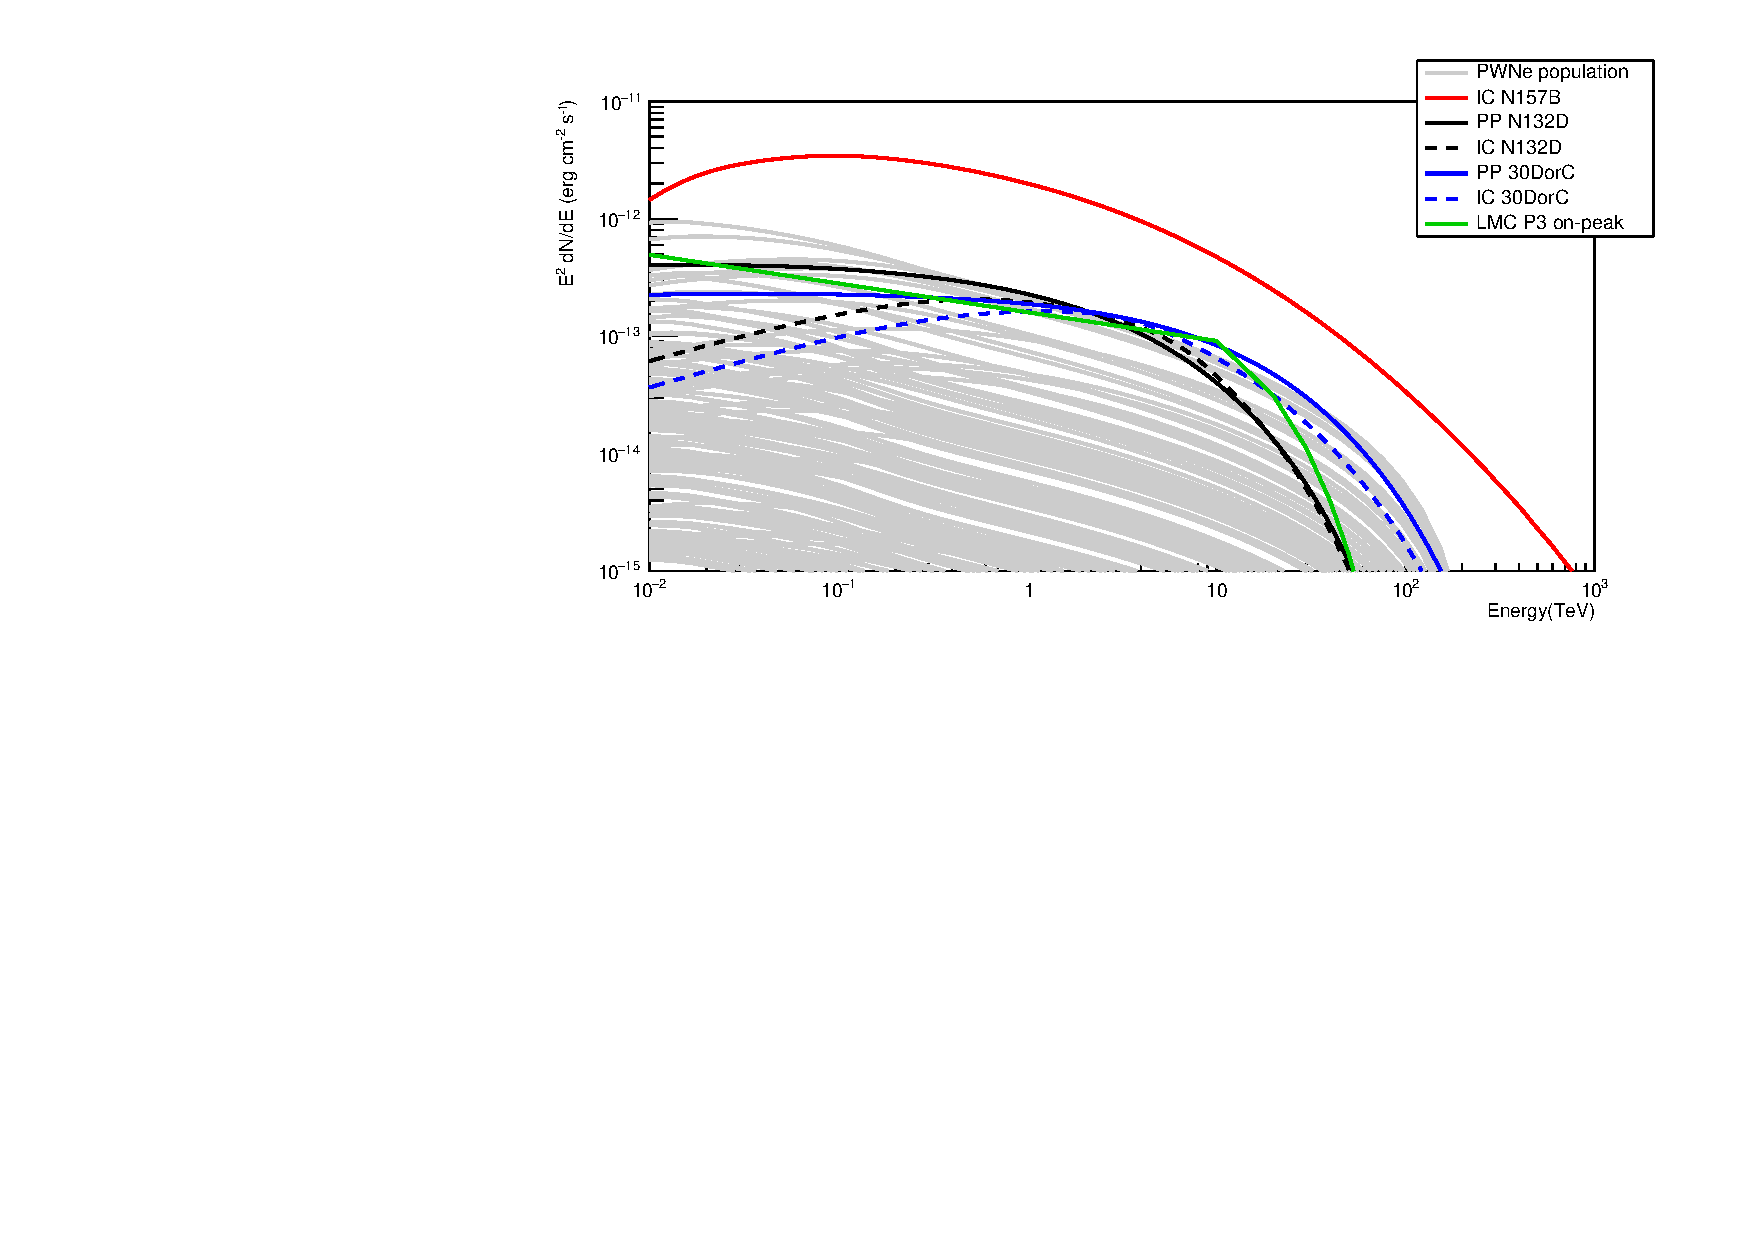
\includegraphics[width=\textwidth]{Pictures/PointSourcesSpec.pdf}
  \caption{\label{fig:PS} Spectral energy distribution of the point sources in the \gls{lmc}. Spectra from N157B, N132D and 30DorC are extracted from \cite{2015HESSTeVLMC}. Spectrum of LMC P3 is a power-law with the spectral parameters of the on-peak orbital region from \cite{2017HESSLMCP3}, with an exponential cut-off at 10 TeV. Spectra from the \gls{pwne} population are derivated following the baseline model described in section \ref{sec:pwnepop}}
\end{figure}

\subsubsection{Supernova Remnant N132D}

Both \textit{Fermi}-LAT and \gls{hess} have detected gamma-ray emission with strong evidences to belong to the \gls{snr} N 132D, a very bright thermal X-ray remnant. It is the brightest remnant of the \gls{lmc} and belongs to a rare type of oxygen-rich remnants which show optical emission from pure heavy-element ejecta, similar to the \gls{mw} \gls{snr} Cas A \cite{2007N132D}. The origin of this \gls{snr}, deduced by its chemical composition, is the core-collapse supernova of a massive progenitor star of $> 35 M_{\odot}$ \cite{2007N132D}. The origin of the gamma-ray emission yields on the interaction of the supernova shock with the cloud of dense material ejected by the progenitor star during its lifetime. The flux detected by \gls{hess} \cite{2015HESSTeVLMC}, with a gamma-ray luminosity in the 1-10 TeV band of $0.9 \pm 0.2 \times 10^{35}(d/50kpc)^2$ erg/s, allow to contemplate the possibility of two possible origins of the radiation: In the hadronic scenario the flux of gamma-rays is produced by the decay of neutral-pions, which would imply a remarkably high fraction of energy injected to cosmic rays by the supernova explosion, or a gas density higher than the one expected from X-ray observations. Either possibility is plausible given the observations in the optical and infrarred bands, which reveals a structure produced by the interaction of the remnant with shocked interstellar gas \cite{2006shockn132D}. In the leptonic scenario, gamma rays are produced by \gls{ic} scattering of low energy-photons. This model could be supported by the high synchrotron radio emission in radio and X-rays, however, it would require a lower magnetic field than the one inferred from radio observations ($20 \mu G$ vs. $40\mu G$). The fluxes and spectral index measured by \textit{Fermi}-LAT in \cite{2016LMCFermiLAT} seem to rule out this model.\\
For this work, we use the hadronic (PP) model shown in figure \ref{fig:PS} based on \gls{hess} measurements.


\subsubsection{Superbubble 30 Dor C}

The Superbubble 30 Dor C, detected by \gls{hess} in the \gls{vhe} range, is a radiation emitting shell which stands out in X-rays, being the largest X-ray synchroton shell known (with a radius of 47pc) \cite{200430dorcxrays}, and also emits radio and optical radiation \cite{1985SNRsintheLMC30dorc}. Its origin seems to be related to the stellar winds and supernovae of the stellar association LH 90 \cite{198430dorLH90}. Both leptonic and hadronic scenario could explain the gamma-ray flux detected by \gls{hess} from this source as discussed in \cite{2015HESSTeVLMC}. The two models are shown in figure \ref{fig:PS}. For this work we tested the both models, knowing that \gls{cta} observations from 100 GeV will be very likely able to set which is the most probable model, thanks to the slope differences up to 1 TeV.

\subsubsection{Binary system LMC P3}

This object was first detected by \textit{Fermi}-LAT at \gls{he} energies in \cite{2016LMCFermiLAT}, but was classified as an unidentified source in the environment of the HII regions NGC 2029/NGC2032. They measured a very soft power-law spectrum (index $\sim 2.8$) but dit not notice any variability down to a monthly basis.
Later, emission from this object in the \gls{vhe} range was detected by \gls{hess} \cite{2017HESSLMCP3}. They discovered a variability of 10.3 period, classifying the object as the first extragañactic gamma-ray binary system. The position of LMC P3 is consistent with a soft X-ray source, which variability of X-ray flux and radial velocity of Balmer absorption lines confirmed that it is very likely a binary system \cite{1981softXraysLMC}, \cite{2012xraybinaryP3}. From optical radial velocity measurements, it is derived that the system must be composed by a neutron star with an O5III star companion \cite{2016P3binary}. Gamma-ray binaries are believed to be a brief phase of the evolution of high-mass X-ray binaries, in which the gamma-ray emission dominates the electromagnetic output \cite{1989binaries}.\\
The spectrum of LMC P3 (HESS J0536-675) was fitted by \gls{hess} to a simple power law of the form $\frac{dN}{dE} = \Phi_{1TeV}\left( \frac{E}{1TeV}\right)^{-\Gamma}$ with an on-peak spectral index $\Gamma$ of 2.1, and an off-peak index of 2.4, where on-peak represents the orbit region where most of the gamma-ray radiation is emitted. The detection of the source only achieved enough statistical significance during the on-peak period.\\
For simplicity in this work, we will assume the on-peak spectral parameters of the source without any temporal modulation ($\Gamma=2.1$, $\Phi_{1TeV} = 5 \cdot 10^{-13}cm^{-2}s^{-1}TeV^{-1}$). The justification is that the on-peak orbital phase lasts for $\sim 50$h, which is way below the total observation time assigned to the \gls{lmc} survey. A test on the possibility of detecting the off-peak emission with \gls{cta} was also carried on and results are given in section \ref{sec:results}.

\subsection{PWNe population in the LMC}\label{sec:pwnepop}

\gls{pwne} are the predominant class of TeV emitters in our Galaxy, with more than 30 sources detected up to date \cite{2009TeVreview}. If we assume that the same is true for the \gls{lmc}, we can model a typical \gls{pwne} population reproducing the so called \textit{baseline} spectral model, first introduced by \cite{2012PWNemodel} and revised by \cite{2018hessPWNe}. The model is a one-zone, time-dependent model which allows to trace the evolution of \gls{vhe} lepton population and hence, radiative output of a \gls{pwn}.
In the model, the number of leptons with energy $E$ residing in the nebula at time $t+\delta t$ will be determined by the balance between the injected leptons and those cooled out the respective energy interval:

\begin{equation}
\frac{dN}{dE}(E, t+\delta t) = \frac{dN_{cooled}}{dE}(E,t) + \frac{dN_{inj}}{dE} (E, t+\delta t)  
\end{equation}

Where for the number of injected leptons $dN_{inj}/dE$ a power-law spectral shapw is assumed:

\begin{equation}
  \frac{dN_{inj}}{dE}(E,t) = \Phi_{0}(t) \left(\frac{e}{1 TeV} \right)^{-\beta}
\end{equation}

with a power-law index $\beta$, also known as injection index. The normalization $\Phi_0(t)$ will depend on the amount of spin-down energy converted into relativistic electrons and positrons in a time step $t+\delta t$.
The cooling mechanisms comprise synchrotron escape and adiabatic losses, and the number of cooled leptons can be approximated by:

\begin{equation}
  \frac{dN_{cooled}}{dE}(E, t) = \frac{dN}{dE} (E, t-\delta t)\cdot exp \left(-\frac{\delta t}{\tau_{eff}(E,t)} \right)
\end{equation}

Where $\tau_{eff}$ is the effective cooling timescale, which will depend on the time evolution of the \gls{pwn} radius and magnetic field strength.\\
The baseline model requires a series of parameters which are listed in table \ref{tab:baselinemodelpwne}:

\begin{table}
  \centering
  \begin{tabular}{llll}
    \hline
    Parameter description & & & Parameter values \\
    \hline
    Braking index & n &  & 3.0 \\
    Initial spin-down power & $\dot E_{0}$ & ($10^{39}$ erg s$^{-1}$) & 2.0 \\
    Initial spin-down timescale &$\tau_{0}$ & (kyr) & 0.5 \\
    Initial magnetic field strength & $B_{0}$ & ($\mu$ G) & 200\\
    Reverse shock interaction timescale & $\tau_{rs}$ & (kyr) & 4.0 \\
    \gls{pwn} radius at t=3kyr & $R_{3}$ & (pc) & 6.0 \\
    Adopted const. \gls{ism} magn. field strength & $B_{ISM}$ &($\mu$ G) & 3.0 \\
    Lepton conversion efficiency & $\eta$ & & 1.0 \\
    Index of magnetic field evolution & $\alpha$ & & 0.6 \\
    Index of letpon injection spectrum & $\beta$ & & 1.75, 2.0, 2.25\\
    Lower bound of lepton energy distribution & $E_{min}$ & (TeV) & 0.03 \\
    Upper bound of lepton energy distribution & $E_{max}$ & (TeV) & 300\\
    \hline
  \end{tabular}
  \caption{Parameters used for the modelling of the \gls{pwne} population, based on table A.1 from \cite{2018hessPWNe}.}
  \label{tab:baselinemodelpwne}
\end{table}

Three equally probable values of the injection index $\beta$ have been considered, and the interstellar magnetic and radiation fields have been adapted to the average conditions in the \gls{lmc}.\\
The population of \gls{pwn} has been generated assuming that pulsars are born at a rate of $r_{CC} = 0.0011 SN yr^{-1}$, in agreement with the assumed rate of \gls{sne} explosion and ratio of core-collapse to thermonuclear \gls{sne}, assuming that all core-collapse \gls{sne} lead to the formation of a spinning neutron star. The lifetime assumed for each \gls{pwn} is of $\tau_{PWN} = 200 kyr$, which yields to an average number of $r_{CC} \times \tau_{PWN} = 220$ \gls{pwne} in the \gls{lmc} if the pulsar creation is assumed to be in steady state during the time $\tau_{PWN}$. The following steps have been carried on to generate the synthetic population of \gls{pwne}:

\begin{itemize}
\item (i) Draw a random number of objects from a Poisson distribution with mean $r_{CC} \times \tau_{PWN}$.
\item (ii) Draw random ages from a uniform distribution over 0 to $\tau_{PWN}$.
\item(iii) Random select an injection index among the three values considered, listed in table \ref{tab:baselinemodelpwne}.
\item (iv) From the baseline spectral model, compute the spectra of all objects given their ages and injection indices.
\item (v) Distribute them sptially among the different massive star forming regions, in proportion to their ionizing luminosity.
\item(vi) Add some luminosity scatter to reflect the properties of the observed \gls{pwne} population in the \gls{mw}.
  \item(vii) Apply two cuts in the synthetic population: First, remove objects younger than 2kyr, because we already know at least two objects of that age (SN 1987A and N158A); second, remove all objects with > 1TeV luminosity above $2.2 \times 10^{34}$ erg s$^{-1}$, because they would have been detected by \gls{hess} already, as shown in the upper limits calculated for SN1987A in \cite{2012HESSLMC}. 
\end{itemize}

The total number of 189 \gls{pwne} have been included in the simulated model, and their spectral energy distributions are shown in figure \ref{fig:PS}.

\section{Simulations and Analysis method} \label{sec:simana}

\subsection{Region of Interest and Observational strategy}

As before mentioned, the  \gls{roi} of the \gls{lmc} extends about 10º in the sky. In order to reach this large \gls{fov}, \gls{cta} will adopt a novel survey mode, which is an observational technique never applied before by \glspl{iact}. It will consist on covering the full region by a series of sightly overlapping pointings with a \gls{fov} of $\sim 3º$ each. The total amount of hours assigned to the \gls{lmc} survey is 340h plus 150h more in case the \gls{snr} 1987A is detected. For this work we have tested different pointing patterns in order to adopt the observational strategy which will maximize the significance of detection both for point sources and extended sources, for a total observation time of 340h. The final scheme consist on 7 pointings of $\sim 1.75 \times 10^5$s each, arranged in 3 rows with a 2-3-2 configuration centered in the coordinates RA=80.0º, dec=-69.0º with a separation of 2º between pointings, as shown in figure \ref{fig:pointings}. In this observation mode, all telescope types of \gls{cta} South are involved.

\begin{figure}
  \centering
  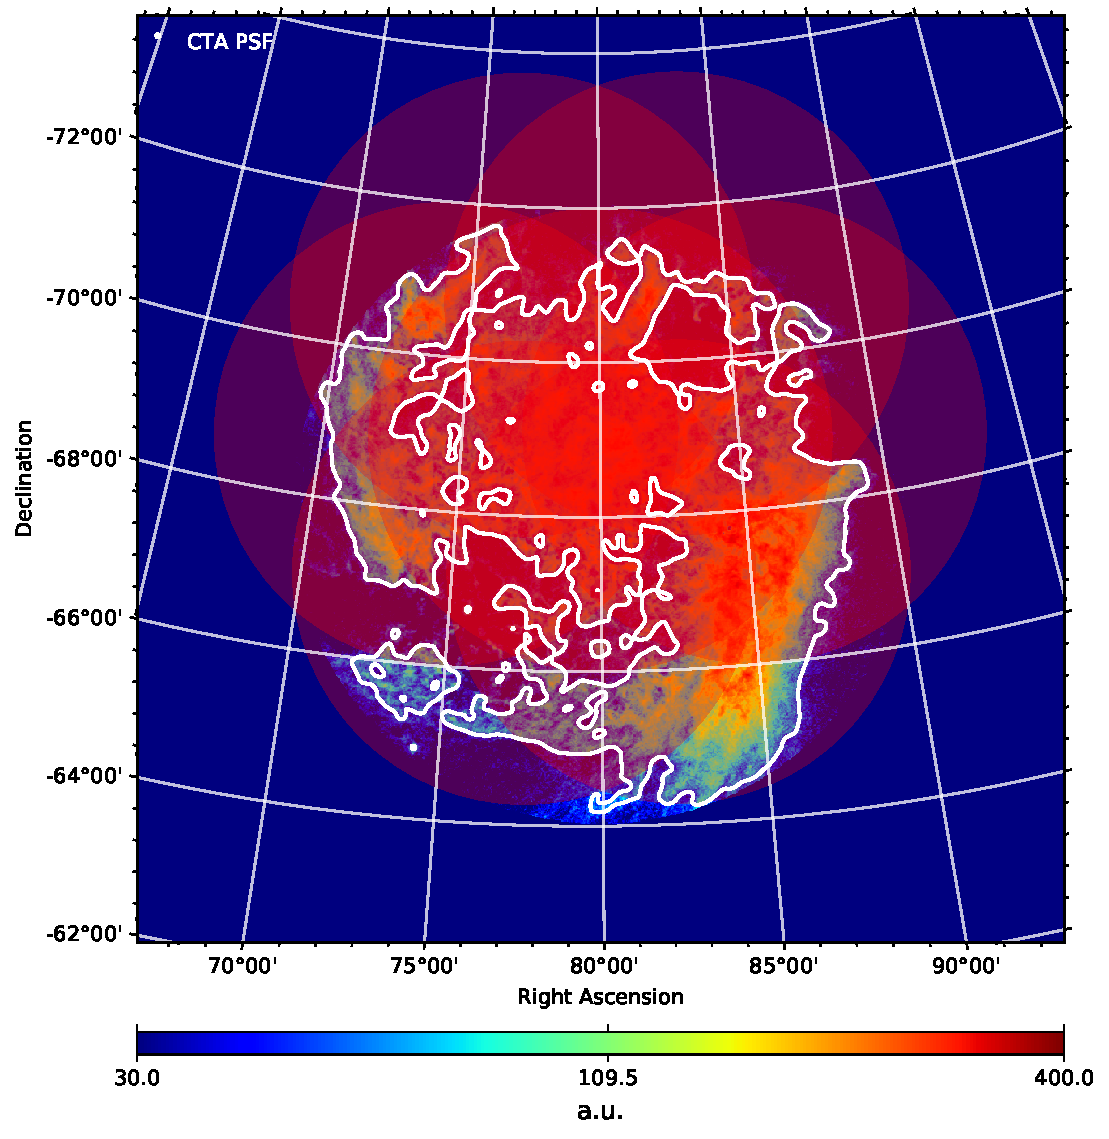
\includegraphics[width=0.7\textwidth]{Pictures/lmc_hi_cdensity_flipped_plot_1000GeV_1TeV.pdf}
  \caption{\label{fig:pointings} Skymap of the region of interest of the \gls{lmc}. The pointing pattern is overlapped in the shape of red circles.}
\end{figure}

\subsection{Simulation parameters}

To calculate the predicted number of counts from a certain emission model, the \gls{cta} collaboration provides a set of \glspl{irf} \cite{CTAPerformance} with information about the effective area and angular resolution of the instrument for several zenith angles. For this work we have used the \gls{irf} \textit{South\_z40\_50h} from the production \textit{prod3b-v2}. This \gls{irf} only accounts for the southern observatory and is optimized for zenith angles around 40º (\gls{lmc} will be seen at $\sim 46$º from the southern site.) and 50h observations. \\
To perform the simulations of the predicted number of counts using the mentioned pointing pattern and \gls{irf} we use \textit{ctools} and \textit{gammalib} \cite{2016Actools}, a software framework for the analysis of astronomical gamma-ray data, specifically designed for \gls{cta}. The tool \textit{ctobssim} uses a MC generator to recreate event lists for observations. As input, it uses a model of the \gls{roi} where each source has a model for the spectral component and for the spatial component, as described in section \ref{sec:model}, and a model of the instrumental background accounting for cosmic-ray events missidentifed as gammas.
Also, \textit{ctobssim} requires the \gls{irf} for the observation and the desired energy range. Each running of \textit{ctobssim} results in a realization of the model where the event list is generated with a random number generator. We have performed realizations of the full emission model of the \gls{lmc} with the pointing pattern described before, in the energy range from 0.05 TeV to 150 TeV. \textit{Ctobssim} is able to combine the different observations of the overlapping pointings, averaging the \glspl{irf} of each region. The resulting event lists are given in FITS file, one for each pointing, which can be combined afterwards for the analysis.\\
The tool \textit{ctmodel} uses the resulting event lists from \textit{ctobssim} and the emission model to calculate an averaged expected number of events. Instead of one realization of the model, it represents the expected number of counts that will be obtained by an infinitely large number of realizations. The result is a counts map, where the averaged number of counts is given for each spatial pixel and for each energy bin. 
The different components of the simulated emission model are shown in picture.
    
\subsection{Fitting method}

We have performed a binned likelihood analysis for this work. We have combined the event lists for the 7 pointings and then we have binned the data into $\sim$ 100 energy bins. The boundaries of the energy bins have been generated using the \textit{ctools} function \textit{csbins}, which inspects the variation in the effective area an background template of the \gls{irf} for the specific simulations, accorting to a threshold settled by the user. To ensure a sufficiently large number of energy bins (it is recommended to have at least 30 bins per decated), the threshold for the fractional change in effective area has been settled to 0.06, and to 0.16 for background rate. \\
The energy range chosen for the analysis is from 100 GeV to 100 TeV. The higher lower limit, compared to the full range of \gls{cta} (which can go down to 30 GeV) comes from the limitations of performance at high zenith angles, given that \gls{lmc} will be always observed at z > 40º.
For the combination of data we have followed the procedure for stacked analysis of \textit{ctools}, where we produce the binned counts map of the data using the function \textit{ctbin} and then we compute the combined background model, the exposure and the point spread function using the functions \textit{ctbkgcube}, \textit{ctexpcube} and \textit{ctpsfcube} respectively. The results are a series of mapcubes which will be used to calculate the maximum likelihood function.\\
A so-called \textit{Asimov} data set has been computed to produce the results presented in this chapter. The \textit{Asimov} data set \cite{2011Asimov} is a representative data set which, when fitted, will retrieve the true values of the model parameters. It can be computed with \textit{ctools} using the function \textit{ctmodel}, and allow to give mean results for significance and upper limits without needing a large number of realizations of the simulated data.

\subsubsection{3D Likelihood Analysis for $\gamma$-ray sources}

The likelihood analysis is based in the typical Poisson likelihood function:
\begin{equation}
  \mathcal{L}(\mu | n) = \prod_{i,j}\frac{\mu_{ij}^{n_{ij}}}{n_{ij}!}e^{-\mu_{ij}}
  \label{eq:likelihood}
\end{equation}

Where $n_{ij}$ represents the 'mock data' counts and $\mu_{ij}$ the model prediction for each bin in energy(i) and space (j). The model $\mu_{ij}$ is the result of the combination of the models for each of the gamma-ray sources described in section \ref{sec:model}. Each source accounts for a spectral model and a spatial model. For extended sources, both components are combined in one mapcube. In the likelihood fitting the only free parameter for each of these models is the normalization $A^{X}$, which determine the relative weight of component $X$. The only exception is the point source LMC P3, which spectral model is a power-law where the free parameters are the normalization and the spectral index. Therefore, the form of $\mu$ is:

\begin{equation}
  \mu_{ij}(A^{X}) = \sum_{X} A^{X} \mu^{X}_{ij}
\end{equation}

The maximum likelihood is calculated finding the normalization parameters $A^{X}$ which maximize equation \ref{eq:likelihood}.
We calculate the significance of a source in terms of the Test Statistics:

\begin{equation}
  TS = 2log \frac{\mathcal{L}(\mu(A^{X})|n)}{\mathcal{L}_{null}}
  \label{eq:ts}
\end{equation}

Where $\mathcal{L}(\mu(A^{X})|n)$ is the maximum likelihood function and $\mathcal{L}_{null}$ is the value of the likelihood function of the null hypothesis for the specific source (making $A^X$ = 0). With this definition, typically a source is considered to be detected when $TS>25$, equivalent to $5\sigma$.\\
The maximum likelihood analysis has been performed using the function \textit{ctlike} from \textit{ctools}. The inputs are the data mapcubes from the stacked analysis and the description of the emission model. We use for the likelihood fit the same emission model used for the simulations. \textit{ctlike} calculates the best fit parameters $A^X$ and the TS values for the requested sources (setting the variable tscalc=''1'').

\subsubsection{Upper limits calculation} \label{sec:ulimits}

For sources which have a flux too low to be detected ($TS < 25$) we calculate upper limits on the minimum flux needed for the source to be detected with \gls{cta}. We calculate this upper limits as the flux that leads to a decrease in the likelihood that corresponds to a certain \gls{cl}. Using the definition of TS from \ref{eq:ts}, according to Wilks' theorem \cite{wilks1938}, TS asymptotically approaches a $\chi^2$-distribution with one degree of freedom under the null hypothesis, therefore to get the flux that yields to the 95\% \gls{cl} upper limit, we must find the normalization parameter $A^X_{max} > A^{X}$ which corresponds to TS = 2.71.\\
This calculation is performed using the function \textit{ctulimit} from \textit{ctools}, which requires as input the mapcube of the mock data and a model with all the sources, including the source for which the upper limit will be calculated. In this case, we use the model resulting from the maximum likelihood fit. Again, the only free parameters are the normalizations. The results from \textit{ctulimit} are the upper limit in the differential flux for a reference energy, the integrated upper flux limit for a specific energy range and the integrated upper energy flux limit for the same range.\\
We have used this method to set constraints on the \gls{dm} annihilation cross section $<\sigma v>$ as described in section \ref{sec:dminlmc}.

\section{Results}\label{sec:results}
        
\subsection{Point sources}

The results for the fitting of the four point sources tested in this work are given in table \ref{tab:fitsources}. The significance of detection of the sources is given in terms of the Test Statistcs described in the previous section. For LMC P3 three cases have been tested: The case of a spectrum following a power-law with the on-peak parameters from \cite{2017HESSLMCP3}; the same power-law but with an exponential cut-off at 10 TeV; and a last case where no source has been simulated, but an upper limit on the flux for a source with the off-peak spectral parameters has been computed.\\
The point sources have been fitted in the full energy range to the same models used for simulation, where the only free parameter is the normalization.
The results show that \gls{cta} will be able to detect with high significance all the known point sources in the \gls{lmc}, including the binary system \gls{lmc} during the on-peak orbital region, and will be able to test the flux of the off-peak region to lower values than the upper limits settled by \gls{hess}. 


\begin{table}
  \centering
  \resizebox{\textwidth}{!}{%
  \begin{tabular}{llllll}
    \hline
    Source name & RA(º) & Dec(º) & Normalization & TS & Significance($\sigma$) \\
     &  &  & $(0.1 - 100 TeV)$ &  &  \\
    \hline
    & & Point Sources & & & \\
    \hline
    N157B/HESS J0537-691 & 84.44 & -69.18 & $1\pm 0.005$ & 130951.51 & 361.9 \\
    N132D/HESS J0525-696 & 81.26 & -69.64 & $1\pm 0.019$ & 5370.19 & 73.3\\
    30DorC/HESS J0535-691 & 83.96 & -69.2 & $0.999 \pm 0.022$ & 4762.83 & 69.0 \\
    LMCP3/HESS J0536-675 & 84.0 & -67.59 & Prefactor: $4.99\pm0.05 \cdot 10^{-19}$ & 27353.83 & 165.4 \\
    (on-peak)&  &  & $(cm^{-2}s^{-1}MeV^{-1})$ &  &  \\
    & &  & Index: $2.1 \pm 0.01 $ &  &  \\
    LMCP3/HESS J0536-675 & 84.0 & -67.59 & Int. flux ulimit: $1.23 \cdot 10^{-13}$ & - & - \\
    (off-peak)&  &  & $(cm^{-2}s^{-1})$ &  &  \\
    \hline
    & & Diffuse emission components & & & \\
    \hline
    LMC Pion-decay & - & - & $1\pm0.185$ & 29.06 & 5.39 \\
    LMC IC & - & - & Int. flux ulimit: $7.33 \cdot 10^{-12}$ & - & - \\
     &  &  & $(cm^{-2}s^{-1})$ &  &  \\
    
    
  \end{tabular}}
  \caption{Results of the fit for the four individual point sources included in the emission model. For the first three sources, the normalization of the spectrum is the only free parameter to fit. For LMCP3, a power-law spectrum with exponential cut-off at 10 TeV has been fitted, acordingly with the results of \cite{2017HESSLMCP3}. For the off-peak region, the upper limit at 99\% \gls{cl} for the integrated flux has been calculated.}
  \label{tab:fitsources}
\end{table}

\subsection{Population of PWNe}

For the fitting of the \gls{pwne} population, a mapcube including all the artificially computed candidates has been used for simulation. Then, a recursive fitting to each candidate, ordered by their luminosity, has been performed to obtain the significance of detection. The recursive fitting is stopped when the significance obtained is less than TS=25, setting a limit on the flux that will be detetable with CTA. The results show that ?? from the total of 189 simulated \gls{pwne} would be detected, giving an estimation of the number of new \gls{pwne} that will be discovered by \gls{cta}. It must be taken into account that this is a very optimistic result, giving that the true spectrum and position of each \gls{pwne} is being used for fitting. In reality, a totally blind search will be performed, scanning the full region in the search for excesses, and assuming a generic spectral shape.

\subsection{Diffuse Emission}

The diffuse emission models for pion-decay and \gls{ic} scattering have been fitted as mapcubes where the only free parmeter left is the normalization. The fit in the full energy range has resulted in a positive detection for the pion-decay component, with a mean TS value of 29.06 (5.39$\sigma$ significance). For the \gls{ic} component, the TS obtained is 0.282, resulting in a non-detection. Upper limits for this model have been calculated instead, giving an upper limit at 99\% confidence level in the integral flux limit of $7.33\cdot10^{-12}$ ph cm$^{-2}$s$^{-1}$ in the range 100 GeV-100TeV.   


\section{Dark Matter annihilation in the LMC} \label{sec:dminlmc}

In this section, forecasts on the detection of an additional component of the diffuse $\gamma$-ray sky in the \gls{lmc}, due to the annihilation of \gls{dm} are developed. The assumption on the \gls{dm} model is that it is composed by stable particles which can annihilate and produce a shower of \gls{sm} particles, which in turn would lead to either direct opr secondary production of $\gamma$-rays, as explained in section \label{sec:DM}. The range of energies for this process can go from a few GeV to several TeV, making it potentially observed by \gls{cta}.\\
It must be taken into account that there exists plenty of \gls{dm} candiates in the literature \cite{2004DMcandidates}, \cite{2005DMcandidates}, \cite{2009DMcandidates}, but in this work the model of \glspl{wimp} is the one explored.\\
The goal is to explore whether \gls{cta} will be able to observe the annihilation of \glspl{wimp} in the \gls{lmc}, or in the negative case,what constraints on \gls{dm} candidates will it set.\\
The flux of $\gamma$-rays produced by \gls{dm} annihilation was presented in equation \ref{eq:flux}, shown again here for convenience:

\begin{equation}
    \frac{d \Phi}{dE}=\frac{1}{8 \pi} \frac{<\sigma v>}{m_{\chi}^2} \frac{d N_{\gamma}}{dE} \int_{\Delta\Omega}\int_{l.o.s} dl \rho^2(\vec{l})
\label{eq:flux}
\end{equation}

Where $dN/dE$ is the spectrum of $\gamma$-rays from annihilation of a pair of dark matter particles, $\langle\sigma v\rangle$ is the thermal velocity averaged annihilation cross section, $m_\chi$ is the \gls{dm} particle mass and $\rho$ is the dark matter density profile. If \gls{dm} particle is not its own antiparticle, equation \ref{eq:flux} should be multiplied by a factor 1/2. \\
Along the full analysis, the mass of the \gls{dm} particle and the annihilation cross section will be treated as free parameters. A single annihilation spectra will be assumed where the branching ratio of the reaction is one, meaning that the entire annihilation happens in a specific channel. The results will be presented in the shape sensitivity curves where the minimum annihilation cross section needed for detection is presented against the mass of the \gls{dm} particle for a specific annihilation channel and \gls{dm} profile.

\subsection{Dark Matter profile in the \gls{lmc}}

The \gls{dm} distribution of the \gls{lmc} can be inferred by the gravitational structure of its disk, following the \textit{rotation curve method}. Assuming circular orbits, the mass of a galaxy enclosed in a certain radius can be calculated thanks to the rotation velocity, $v_{rot}$ = GM(<r)/r. Measurements of the rotation velocities of stars and gas in the \gls{lmc} allow to calculate the total mass \cite{LMCHI}, and substracting the contribution to the rotation curve of the luminous matter, the remaining \gls{dm} can be estimated. The dark matter profiles used in this section rely on the works of \cite{2015FermiLMCDM}, where the gas mass component of HI+He as a function of the radius is taken from \cite{1992gasLMC}; and the stellar mass is extracted from \cite{2006LMCkinematics}. The rotation curve of the \gls{lmc} can be seen in picture \ref{fig:rotcurve}.\\
A generalized six-parameter Hernquist-Zhao \gls{dm} profile has been adopted for this work \cite{1990Hernquist}, \cite{1996Zhao}, following equation \ref{fig:gnfw} already shown in section \ref{sec:DM}, repeated here for convenience:


\begin{equation}
    \rho(r) = \frac{2^{\frac{\beta-\gamma}{\alpha}} \times \rho_{0}}{\left(\frac{r}{r_{S}}\right)^{\gamma}\left[ 1+\left(\frac{r}{r_{S}} \right)^{\alpha}\right]^{\frac{\beta-\gamma}{\alpha}}}\Theta(r_{max}-r)
\end{equation} \label{fig:gnfw}

Where $\Theta$ is the Heaviside step function, $r_{S}$ is the scale radius and $\rho_{0}$ is the characteristic density. These two last parameters depend on the specific \gls{dm} halo. Setting $(\alpha,\beta,\gamma) = (1,3,1)$ we retrieve the \gls{nfw} profile \cite{NFW}, with a cusp. An isothermal profile, with a core rather than a cusp is obtained setting $(\alpha,\beta,\gamma) = (2,2,0)$. Variations of these two kinds of profiles have been tested, with parameters shown in table \ref{tab:dmprofiles} and plotted in figure \ref{fig:dmprofiles}. 

\begin{figure}
  \centering
  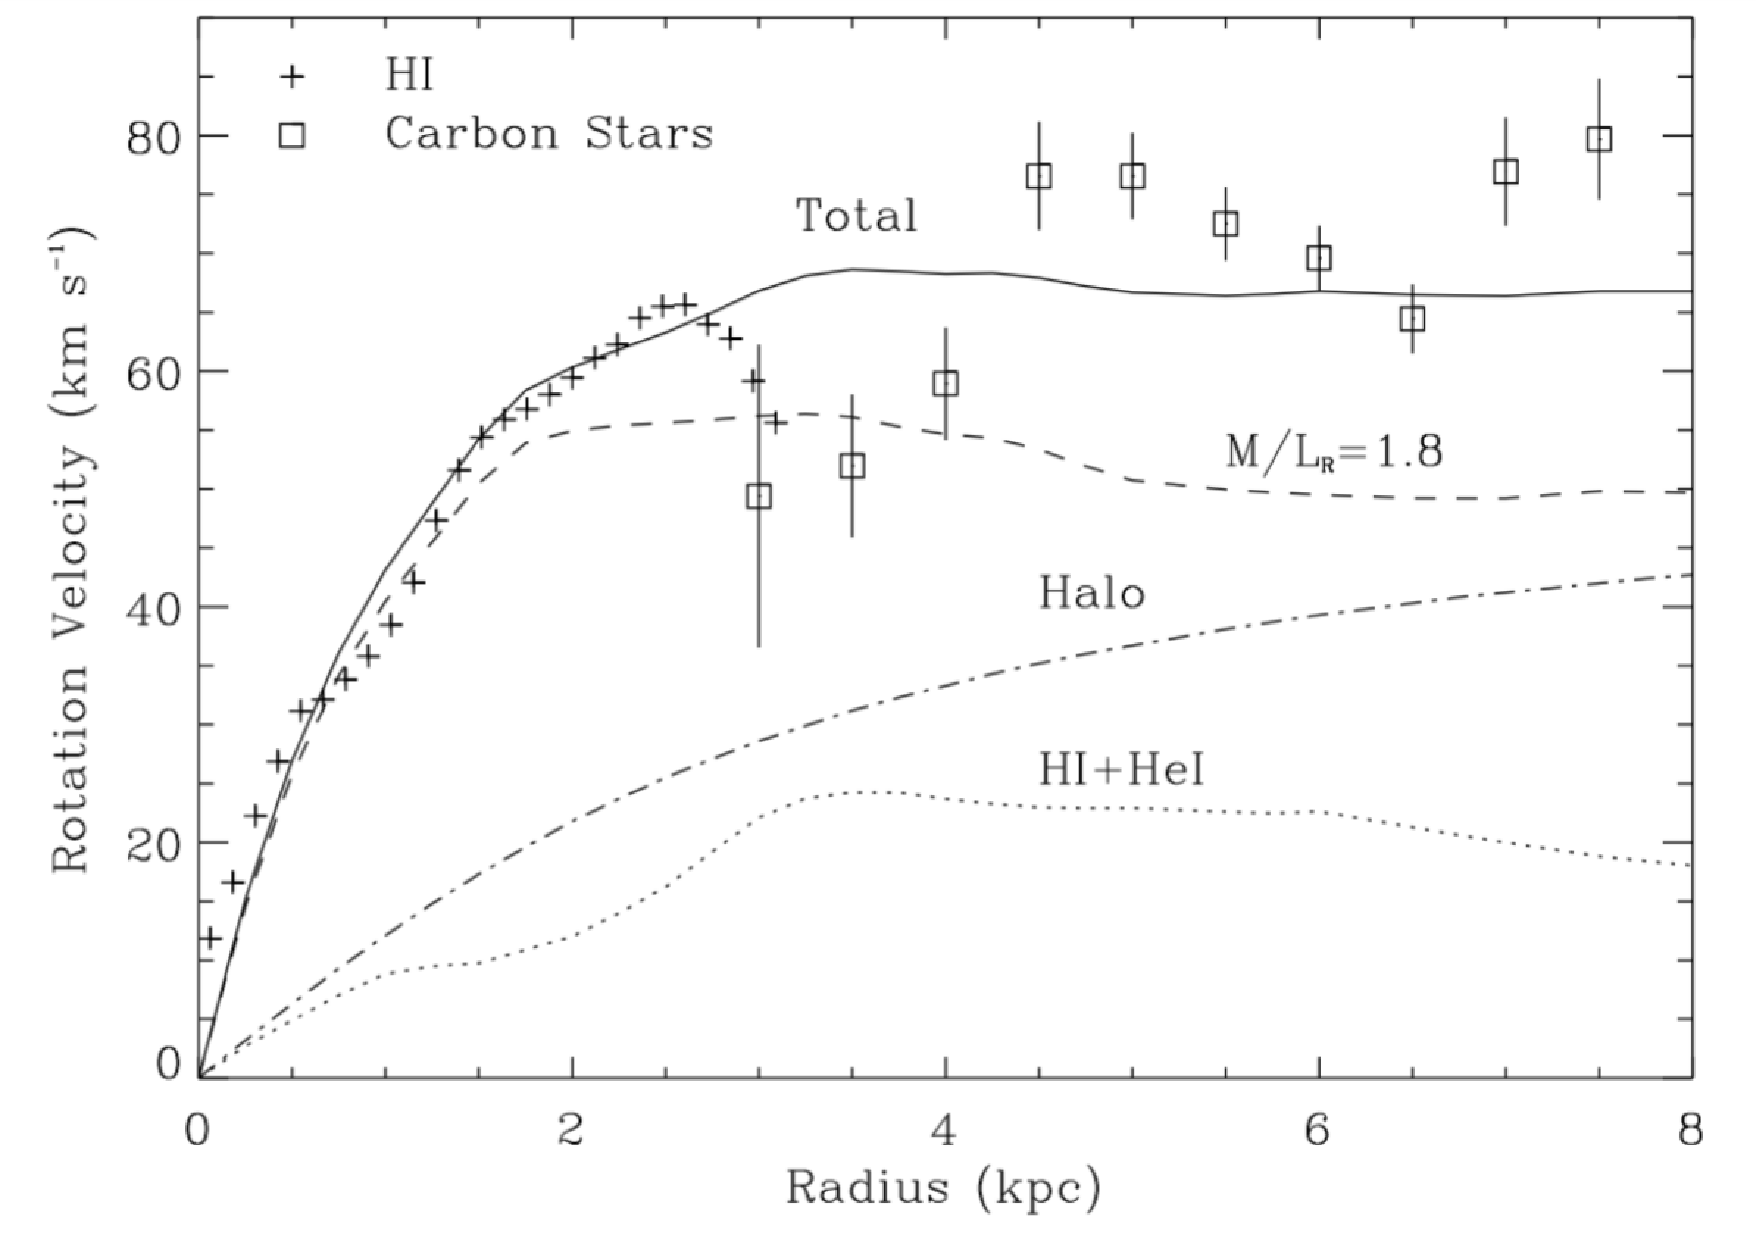
\includegraphics[width=0.7\textwidth]{Pictures/rotationcurvelmc.pdf}
  \caption{\label{fig:rotcurve} Rotation curve of the \gls{lmc}, from \cite{LMCHI}. The solid black line is the total predicted rotation curve constructed from the following components: (\textit{a}) HI mass distribution from \cite{1992gasLMC}, and a 30\% He contribution (\textit{dotted line}). (\textit{b}) R stellar light distribution based on the data from \cite{1958starsinLMC} and $M/L_{R}=1.8$ (dashed line). (\textit{c}) Pseudoisothermal dark halo with core radius 2.5 kpc and central densiy $0.009 M_{\odot}$pc$^{-3}$.}
\end{figure}

\begin{figure}
  \centering
  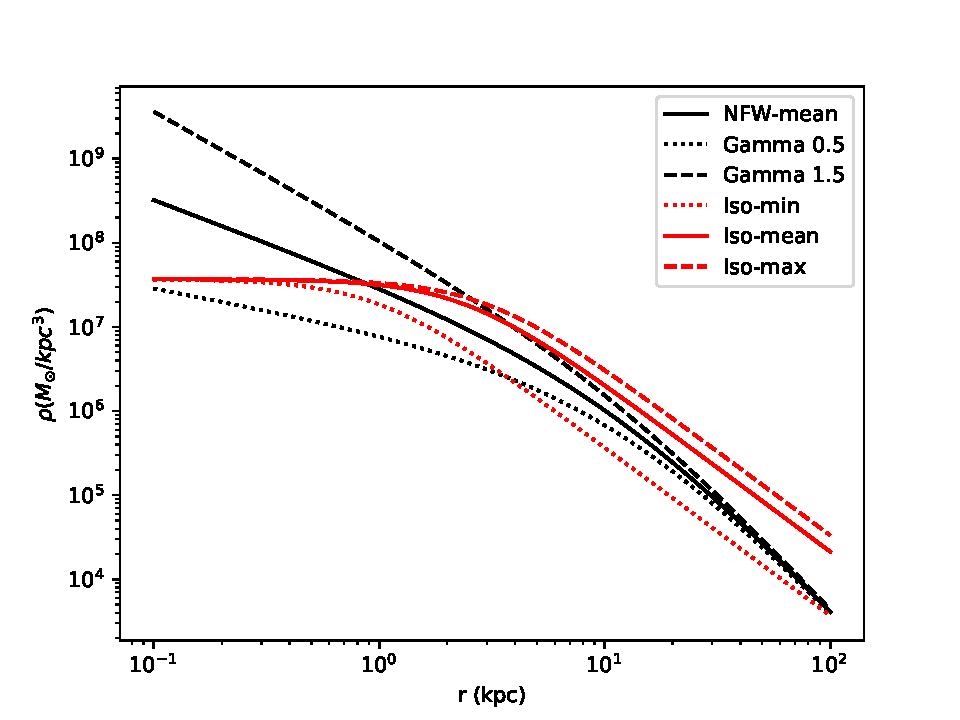
\includegraphics[width=0.7\textwidth]{Pictures/dmprofiles.pdf}
  \caption{\gls{dm} profiles plotted against the radius $r$ from the \gls{lmc} center, with the parameters listed in table \ref{tab:dmprofiles}.} \label{fig:dmprofiles}
\end{figure}

\begin{table}
  \centering
  \resizebox{\textwidth}{!}{%
    \begin{tabular}{llllllll}
      \hline
      Profile & $\alpha$ & $\beta$ & $\gamma$ & $r_{S} (kpc)$ & $\rho_{0} (M_{\odot}/kpc^3)$ & $J (GeV^{2}/cm^5)$ & Field of View(º) \\
      \hline
      NFW-mean & 1 & 3 & 1 & 12.6 & $2.6\times10^6$ & $8.5\times 10^{19}$ & 10 \\
      Gamma0.5 & 1 & 3 & 0.5 & 12.6 & $2.6\times10^6$ & $2.9\times 10^{19}$ & 10 \\
      Gamma1.5 & 1 & 3 & 1.5 & 12.6 & $2.6\times10^6$ &1.0 $\times 10^{20}$ & 10\\
      Iso-min & 2 & 2 & 0 & 1 & $3.7\times10^7$ & $2.3\times 10^{20}$ & 20 \\
      Iso-mean & 2 & 2 & 0 & 2.4 & $3.7\times10^7$ & $2.9\times 10^{20}$ & 20 \\
      Iso-max & 2 & 2 & 0 & 3 & $3.7\times10^7$ & $8.5\times 5.4^{20}$ & 20 \\
    \hline
    \hline      
    \end{tabular}}
    \caption{Parameters of the \gls{dm} profiles used in this work. Values of NFW-mean and Iso-mean profiles are the same as of \cite{2015FermiLMCDM}. The $J$-factors are integrated in the \gls{fov} indicated by the last column.} \label{tab:dmprofiles}
\end{table}

The \gls{dm} profiles were simulated using the software \textit{clumpy}, a code for $\gamma$-ray and neutrino signals from \gls{dm} structures \cite{2019CLUMPY}. It allows to compute simulations of \gls{dm} halos characterized by a series of parameters depending on the \gls{dm} profile. \textit{Clumpy} was used in this work to simulate maps of the J-factor in the region of the \gls{lmc} in order to create the spatial distribution of the different \gls{dm} models, which afterwards were combined with the spectra of several annihilation channels to reproduce the $\gamma$-ray flux in the \gls{lmc}. 
The 2D J-factor of the different profiles used in this work, compute with \textit{clumpy} can be seen in figure \ref{fig:jfactors}.

\begin{figure}
\centering
\minipage{0.5\textwidth}
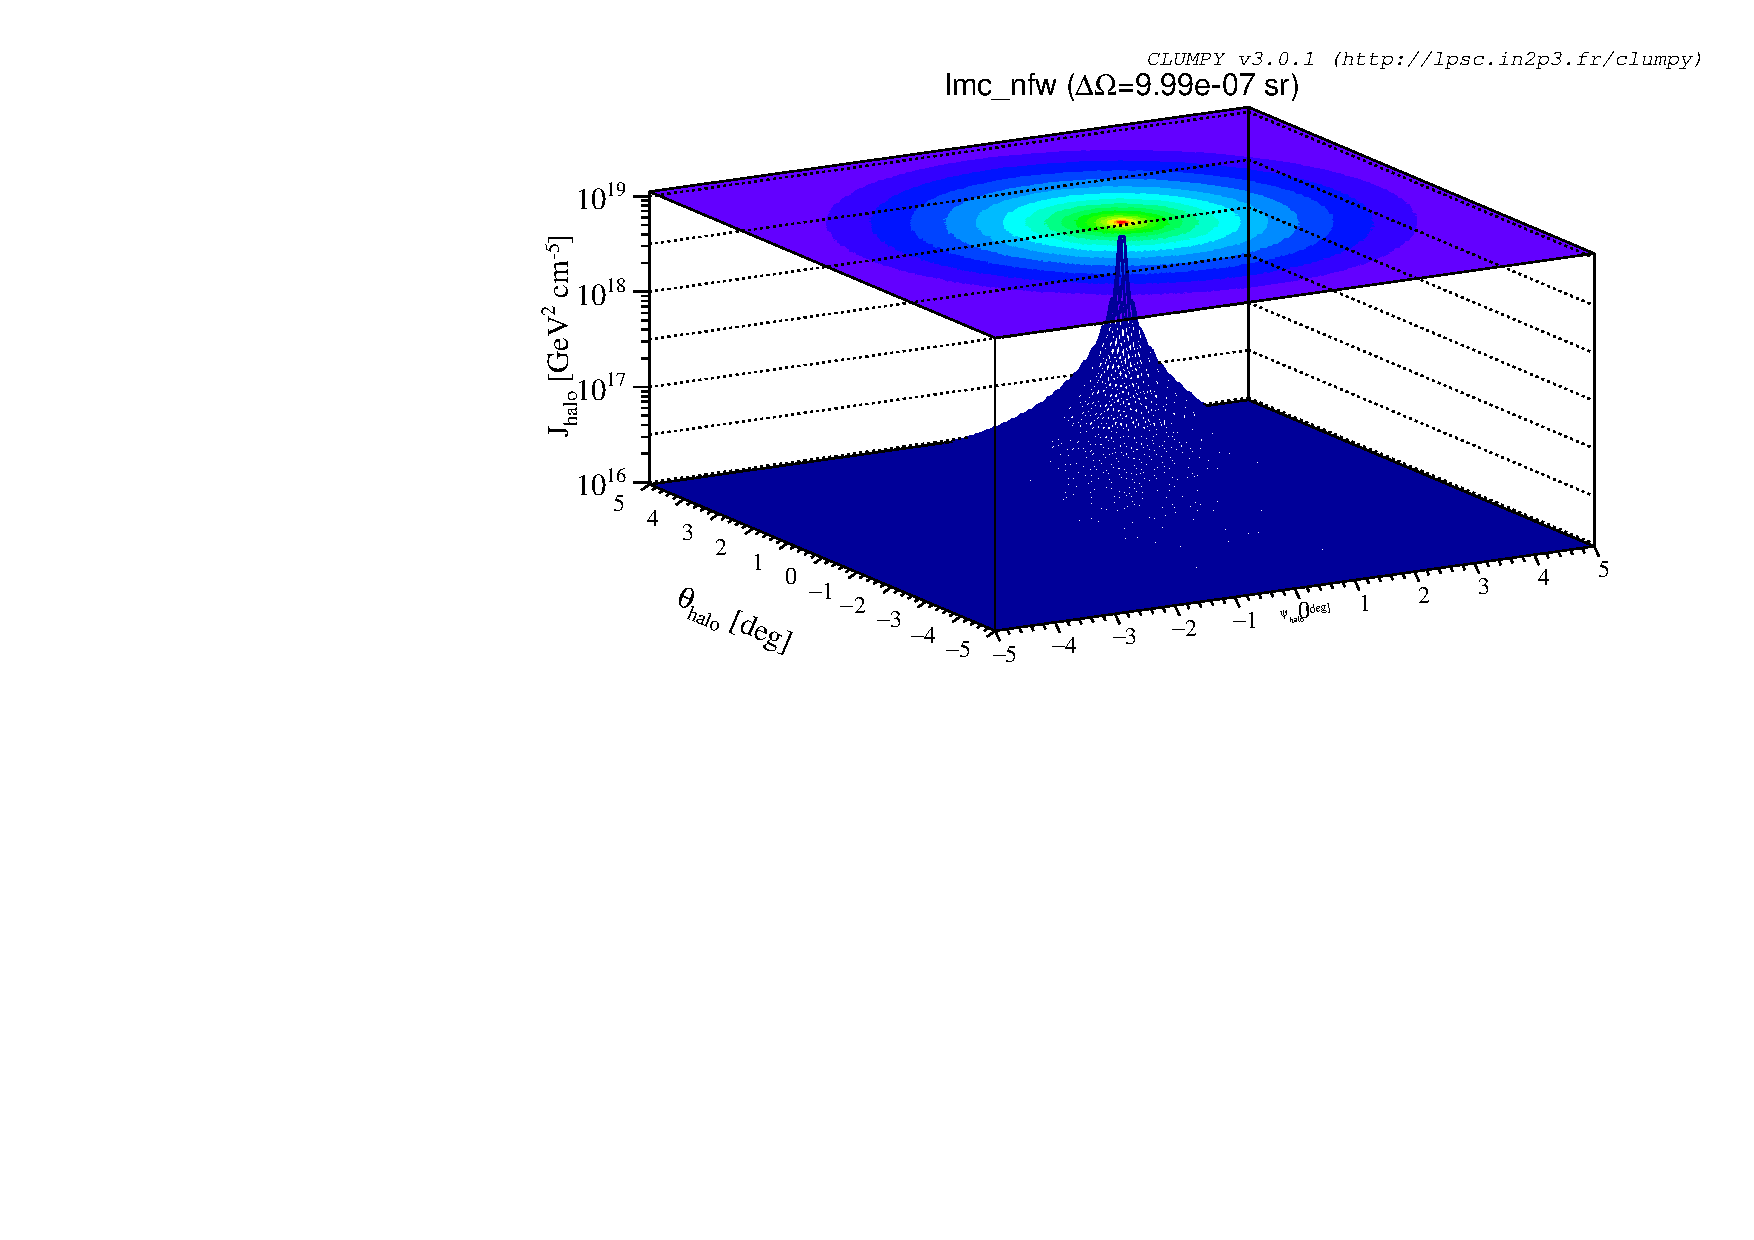
\includegraphics[width=1\textwidth]{Pictures/lmc_nfw.pdf}
\endminipage 
\minipage{0.5\textwidth}
\includegraphics[width=1\textwidth]{Pictures/lmc_iso-mean.pdf}
\endminipage \\
\minipage{0.5\textwidth}
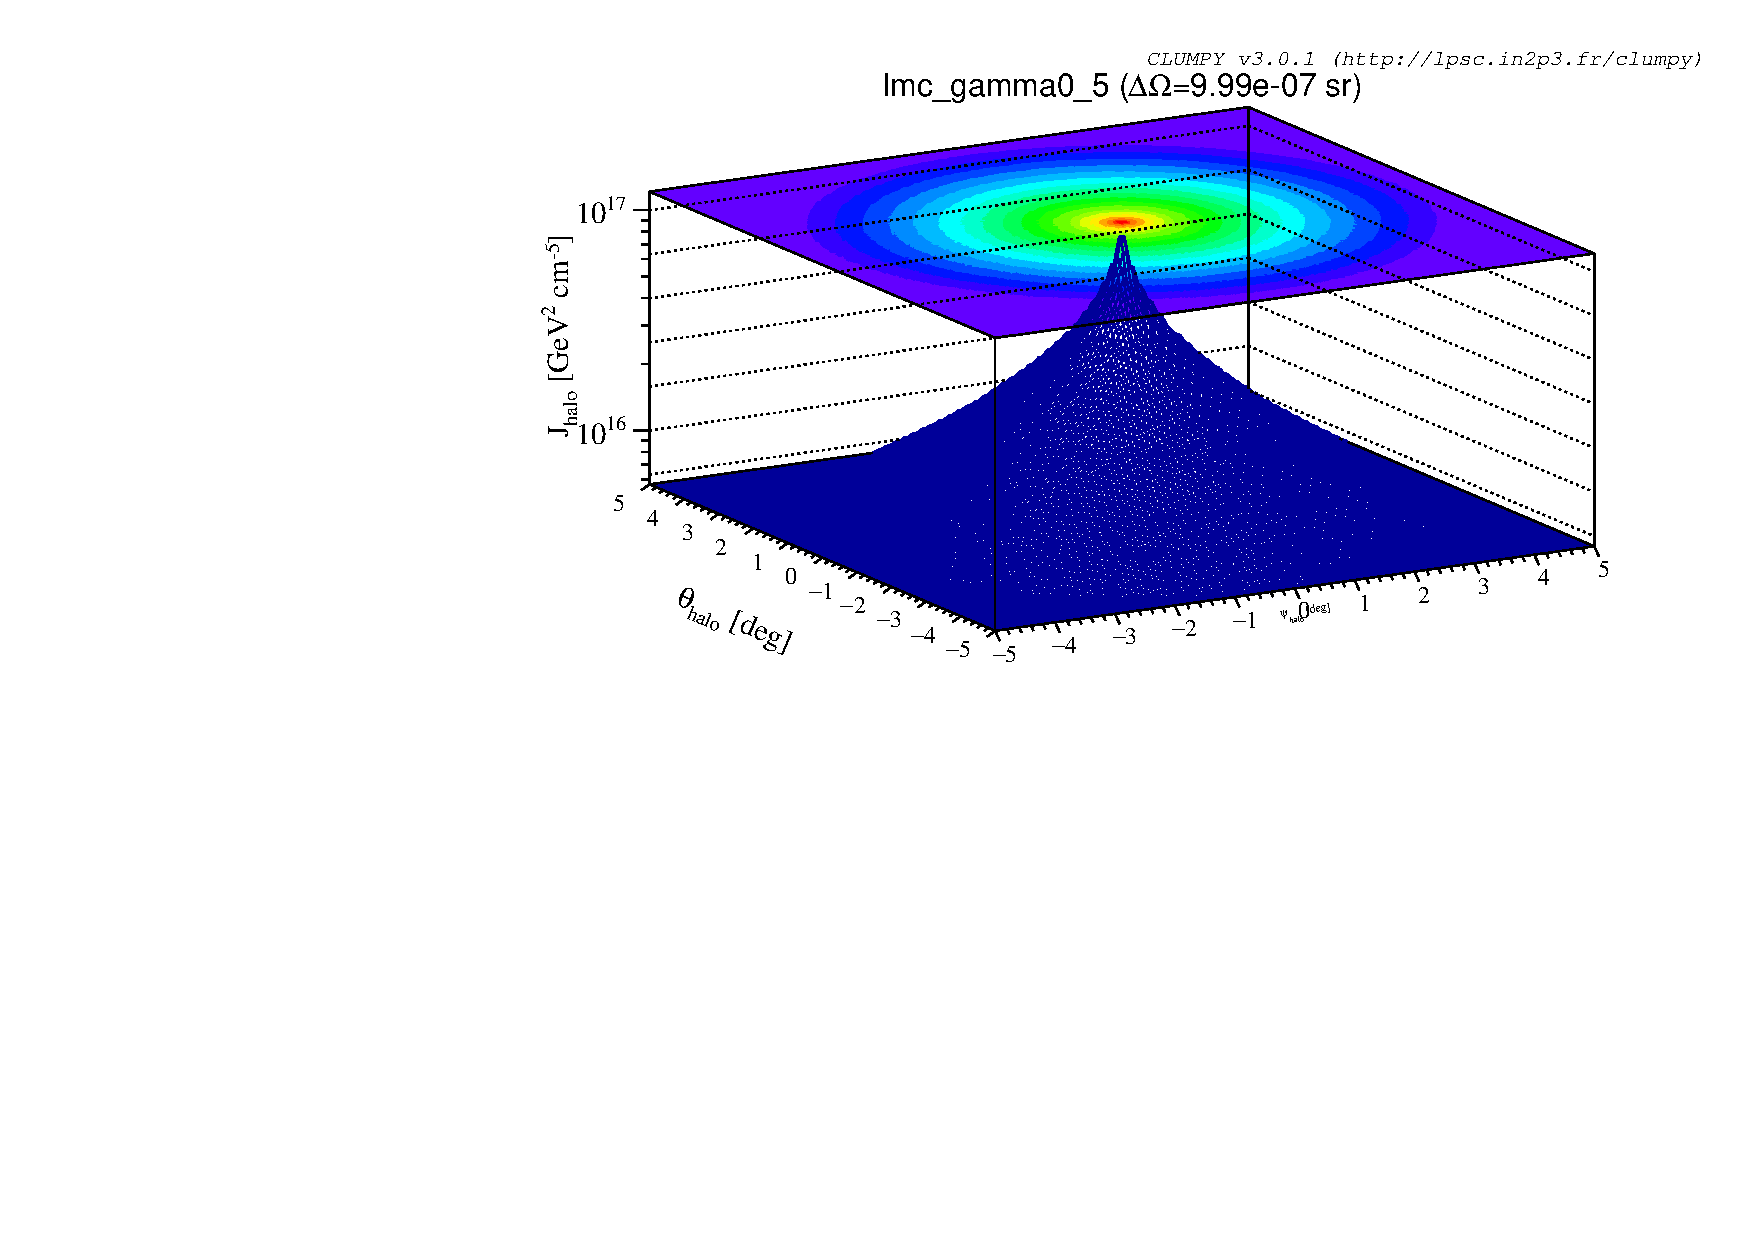
\includegraphics[width=1\textwidth]{Pictures/lmc_gamma0-5.pdf}
\endminipage
\minipage{0.5\textwidth}
\includegraphics[width=1\textwidth]{Pictures/lmc_iso-min.pdf}
\endminipage \\
\minipage{0.5\textwidth}
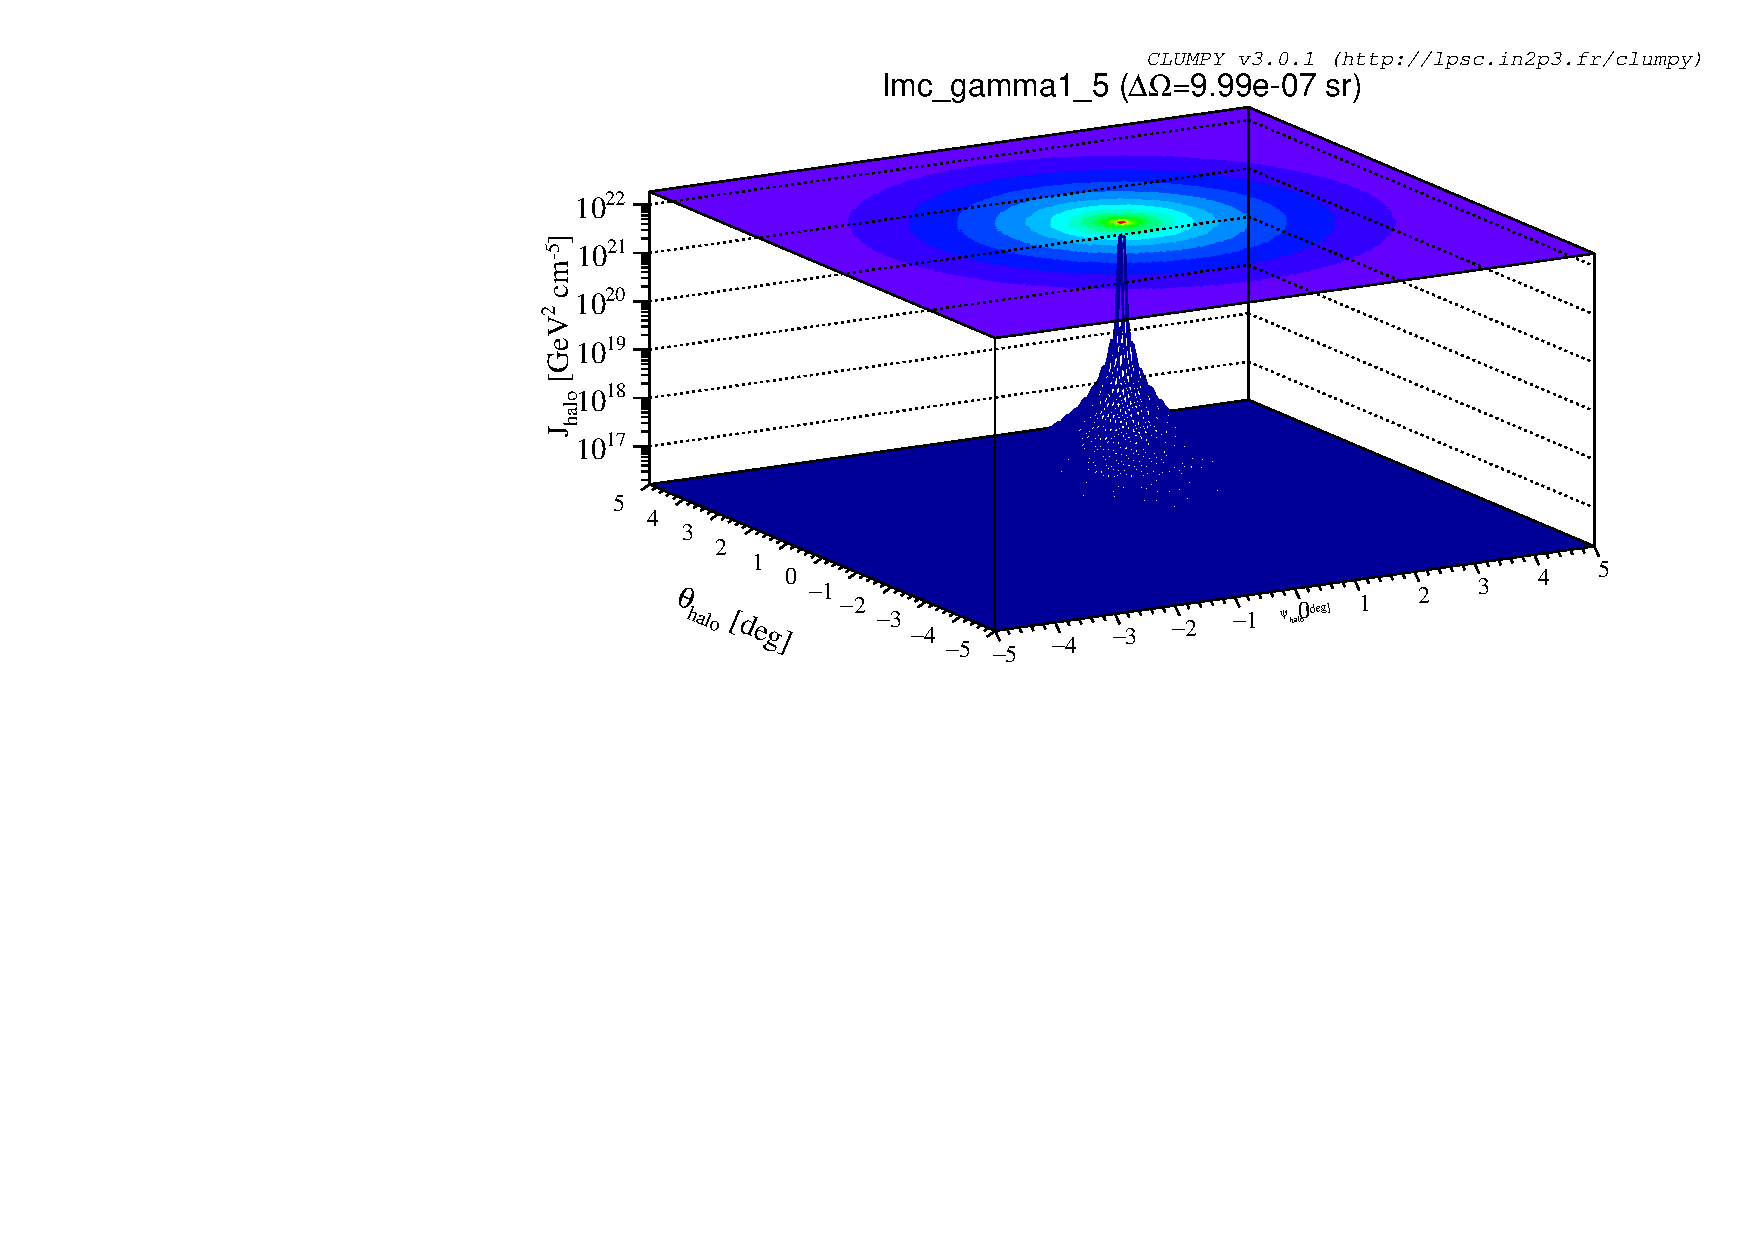
\includegraphics[width=1\textwidth]{Pictures/lmc_gamma1-5.pdf}
\endminipage
\minipage{0.5\textwidth}
\includegraphics[width=1\textwidth]{Pictures/lmc_iso-max.pdf}
\endminipage
  \caption{2-D J-Factors of the \gls{lmc} \gls{dm} profiles probed in this work. The \gls{nfw} and Isothermal profiles were computed using the same parameters as in \cite{2015FermiLMCDM}.}
    \label{fig:jfactors}
\end{figure}

\subsection{$\gamma$-ray spectrum}

For the spectral part of the \gls{dm} emission model ($dN_{\gamma}/dE$ in equation \ref{eq:flux}), the recipes from \cite{2011cirelli} were used, where the energy spectra of $\gamma$-rays produced by different \gls{dm} annihilation channels are provided. For this thesis, the studied channels were $b \overline b$, $W^+ W^-$, $\tau^+\tau^-$, $\mu^+ \mu^-$ including electro-weak corrections as computed in \cite{2011EWcorrections}, and their spectra can be seen in figure \ref{fig:dmspec}, computed for a set of \gls{dm} particle masses.

\begin{figure}
  \centering
  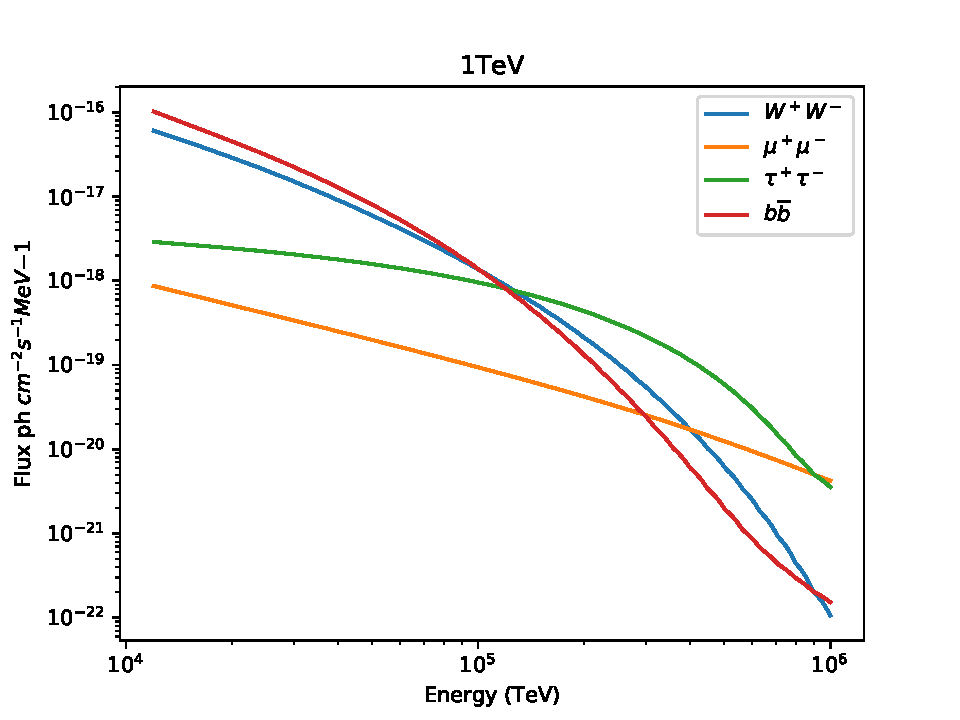
\includegraphics[width=0.6\textwidth]{Pictures/1tevspectra.pdf}
  \minipage{0.5\textwidth}
  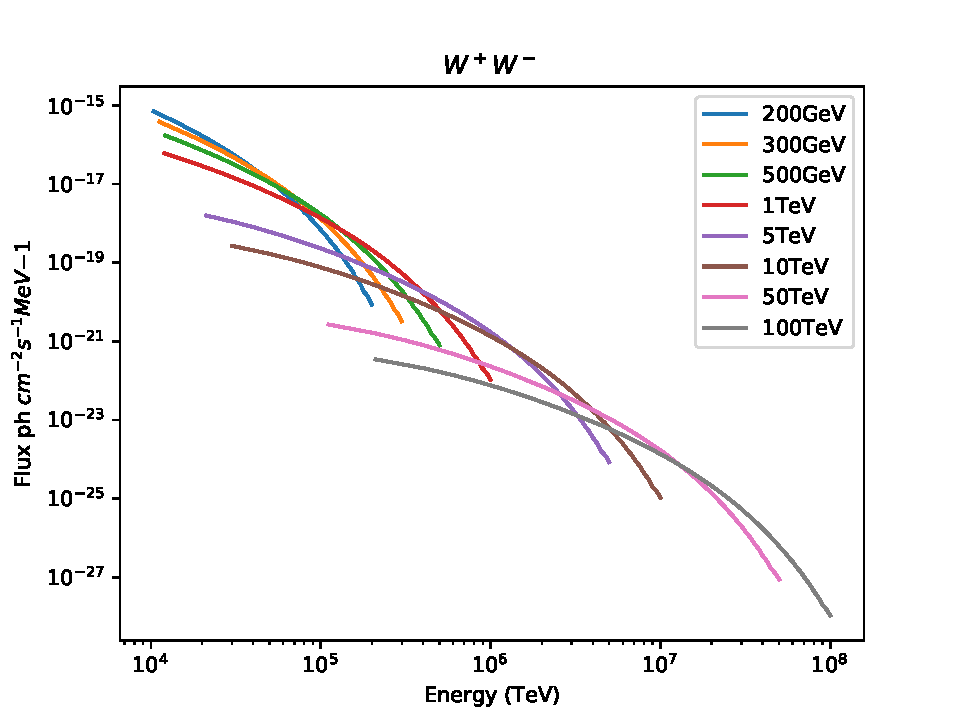
\includegraphics[width=1\textwidth]{Pictures/specW.pdf}
  \endminipage 
  \minipage{0.5\textwidth}
  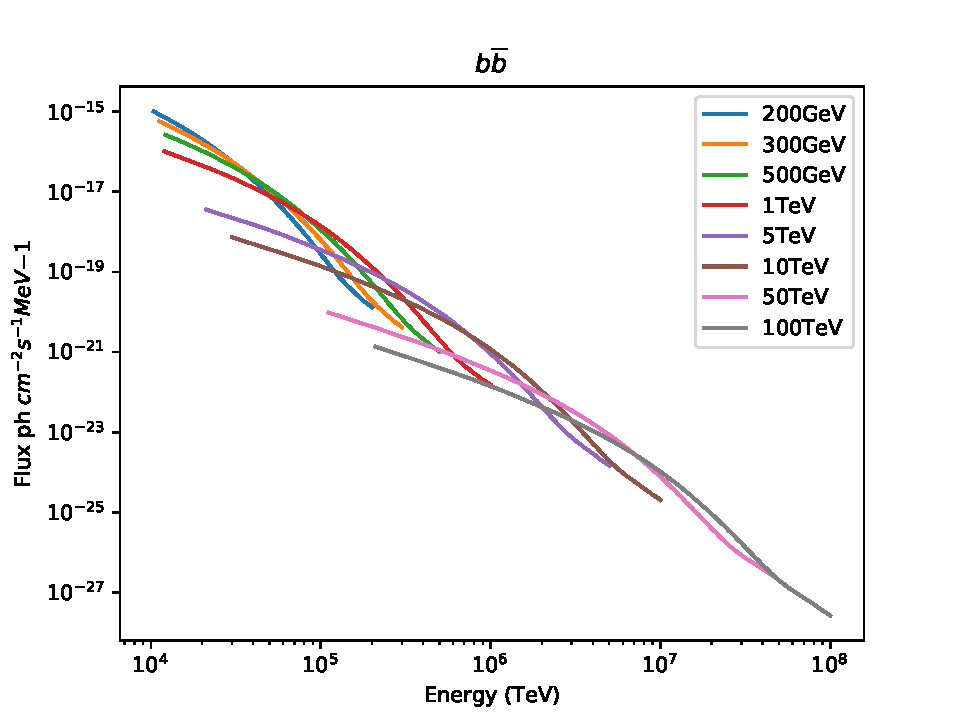
\includegraphics[width=1\textwidth]{Pictures/specb.pdf}
  \endminipage \\
  \minipage{0.5\textwidth}
  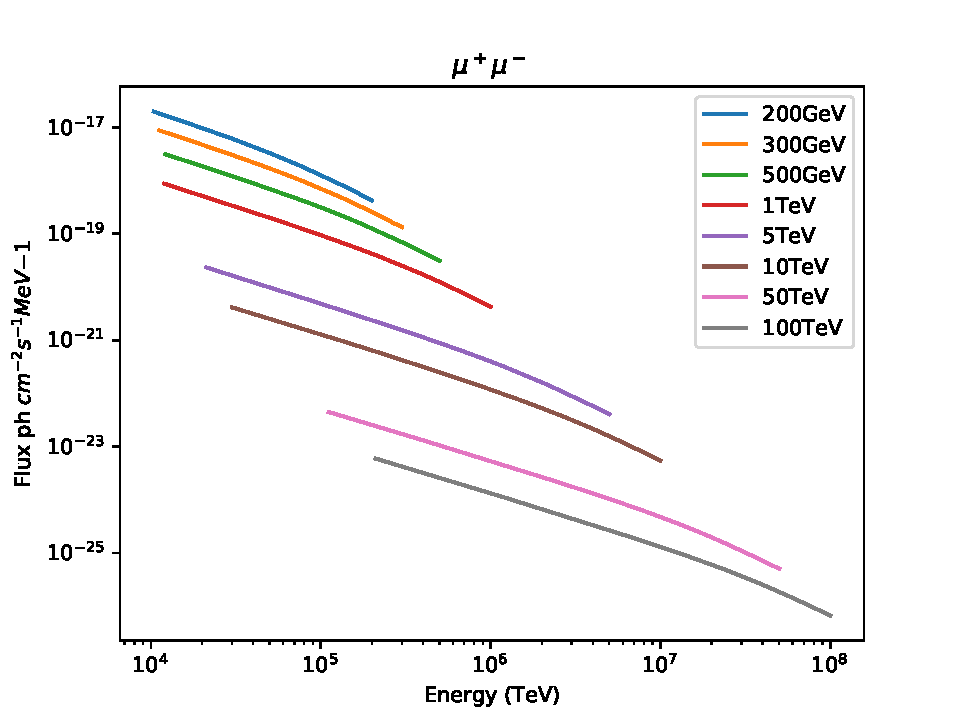
\includegraphics[width=1\textwidth]{Pictures/specMu.pdf}
  \endminipage
  \minipage{0.5\textwidth}
  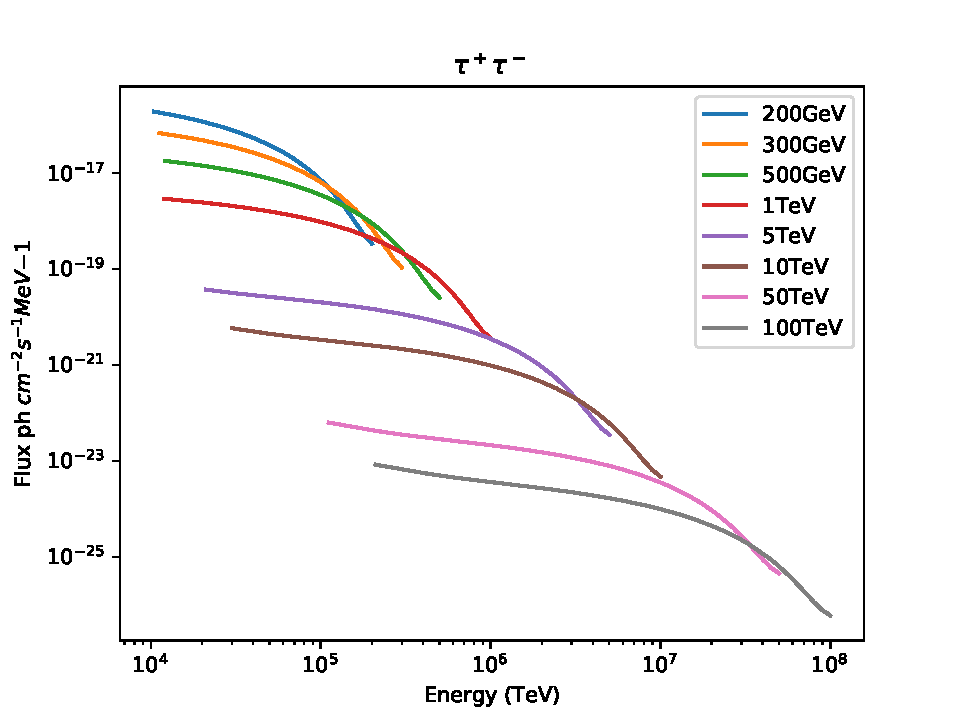
\includegraphics[width=1\textwidth]{Pictures/specTau.pdf}
  \endminipage \\
  \caption{$\gamma$-ray spectra of \gls{dm} pair annihilation, for different annihilation channels and masses of \gls{dm} particle. }
  \label{fig:dmspec}
\end{figure}

\subsection{Results on \gls{dm} sensitivity curves}

Using the \gls{dm} profiles and spectra described in previous section, a likelihood analysis was performed to obtain the minimum flux needed for the \gls{lmc} \gls{dm} component to be detectable by \gls{cta}. The asimov data set with the astrophysical $\gamma$-ray sources described in section \ref{sec:model} is used for this task as a background on top of which we calculate the flux needed to be emitted by each \gls{dm} model in order to be detected. To do so, the procedure for upper limits calculation described in section \ref{sec:ulimits} is applied. Each \gls{dm} model is included in the fitted model as a new source, for which the differential upper flux limit for a reference energy, the integrated upper flux limit over the energy range 0.1 GeV-\gls{dm} particle mass, and the integrated energy limit are calculated.\\
From the resulting flux $\frac{d \Phi_{ulim}}{dE}$, using equation \ref{eq:flux}, the velocity averaged annihilation cross section $<\sigma v>$ can be extracted. The sensitivity curves where $<\sigma v>$ plotted versus \gls{dm} particle masses are shown in figure \ref{fig:dmsensicurves}. Each curve corresponds to a specific \gls{dm} profile and annihilation channel. The space above the curves represent the parameter space of $<\sigma v>$ and \gls{dm} mass that could be detected by \gls{cta}.

\begin{figure}
\centering
\minipage{0.5\textwidth}
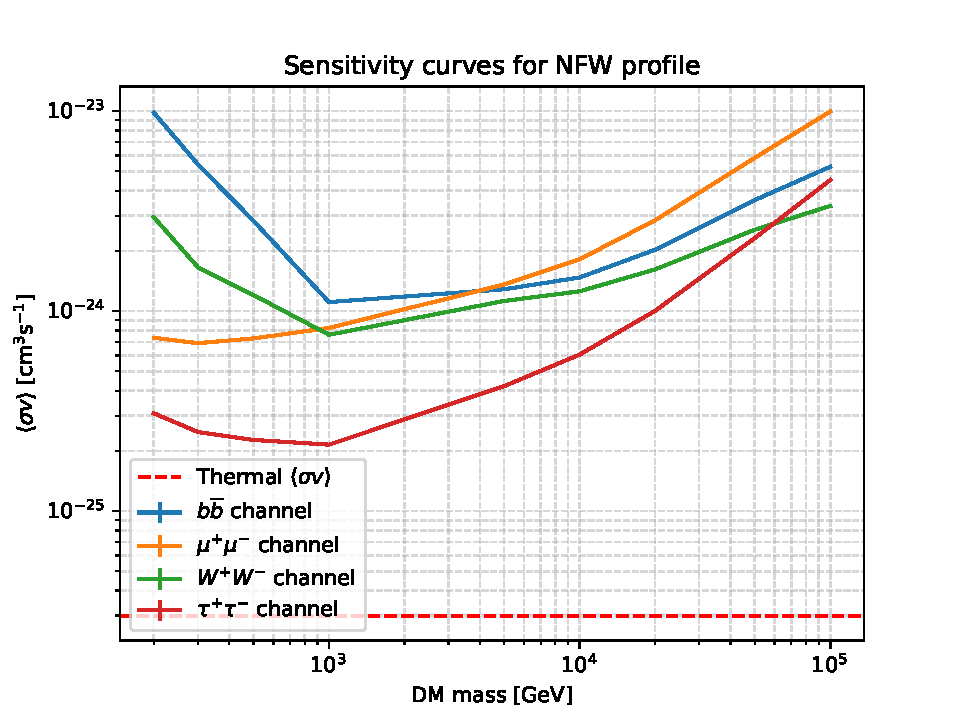
\includegraphics[width=1\textwidth]{Pictures/Limits_NFW.pdf}
\endminipage 
\minipage{0.5\textwidth}
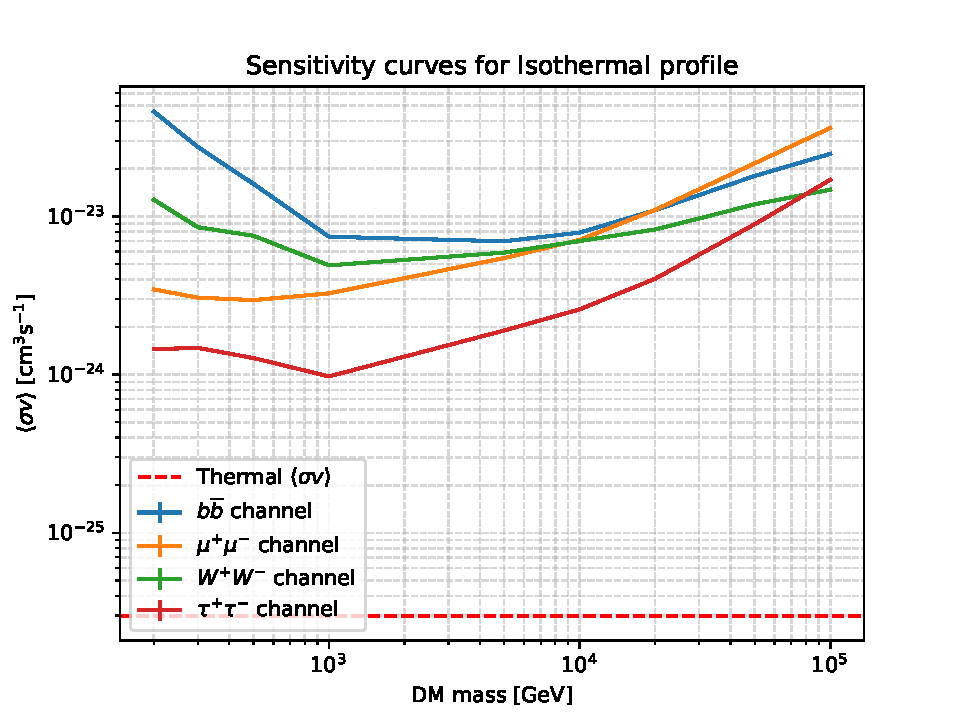
\includegraphics[width=1\textwidth]{Pictures/Limits_Isothermal.pdf}
\endminipage \\
\minipage{0.5\textwidth}
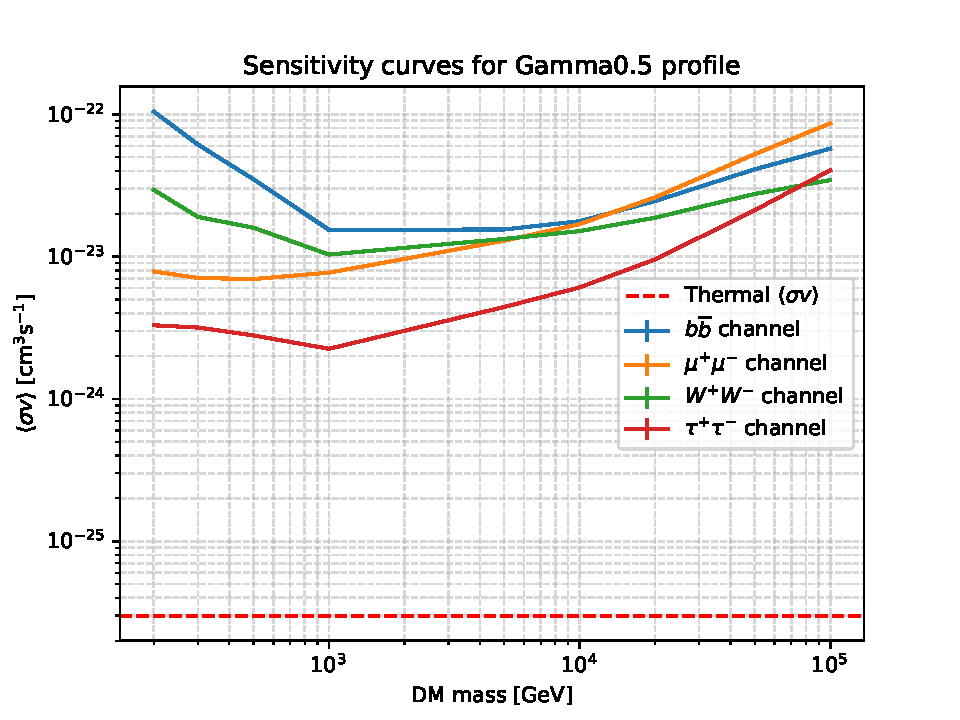
\includegraphics[width=1\textwidth]{Pictures/Limits_Gamma0-5.pdf}
\endminipage
\minipage{0.5\textwidth}
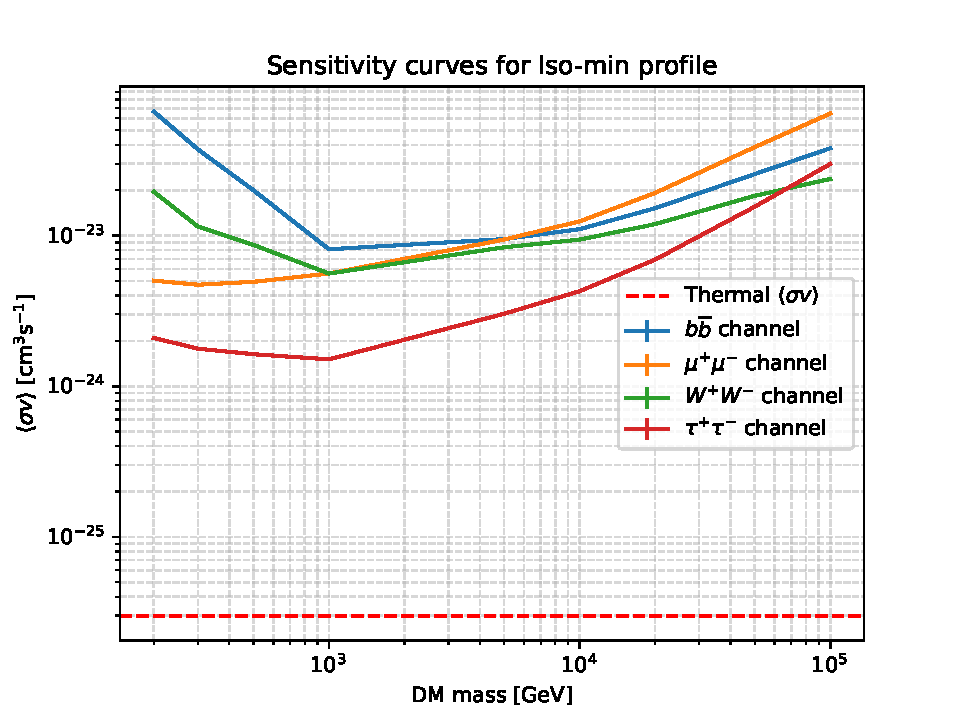
\includegraphics[width=1\textwidth]{Pictures/Limits_Iso-min.pdf}
\endminipage \\
\minipage{0.5\textwidth}
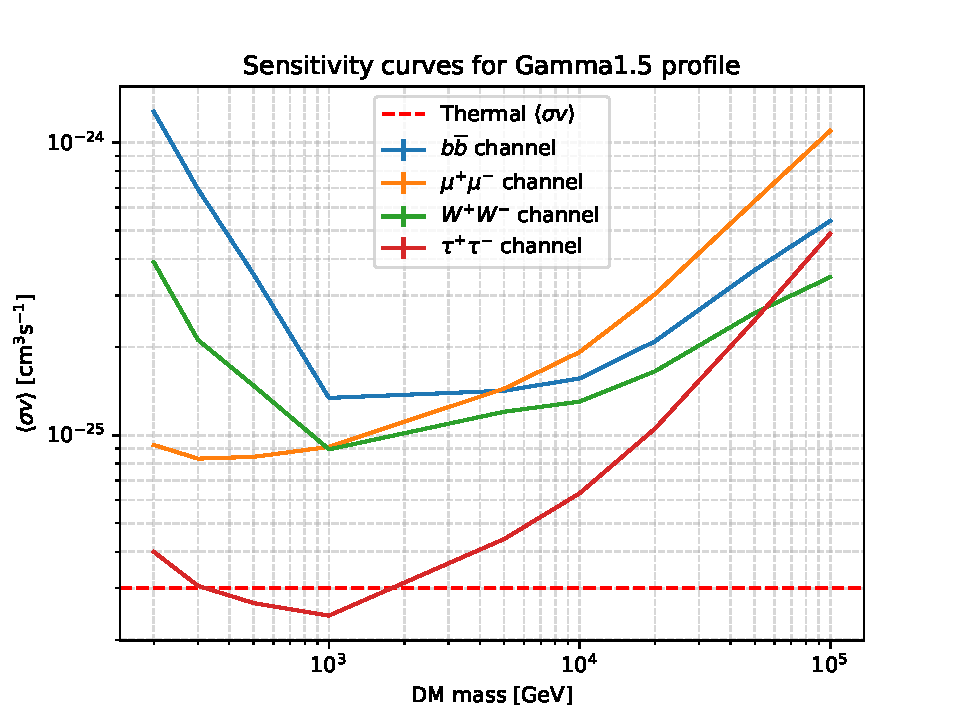
\includegraphics[width=1\textwidth]{Pictures/Limits_Gamma1-5.pdf}
\endminipage
\minipage{0.5\textwidth}
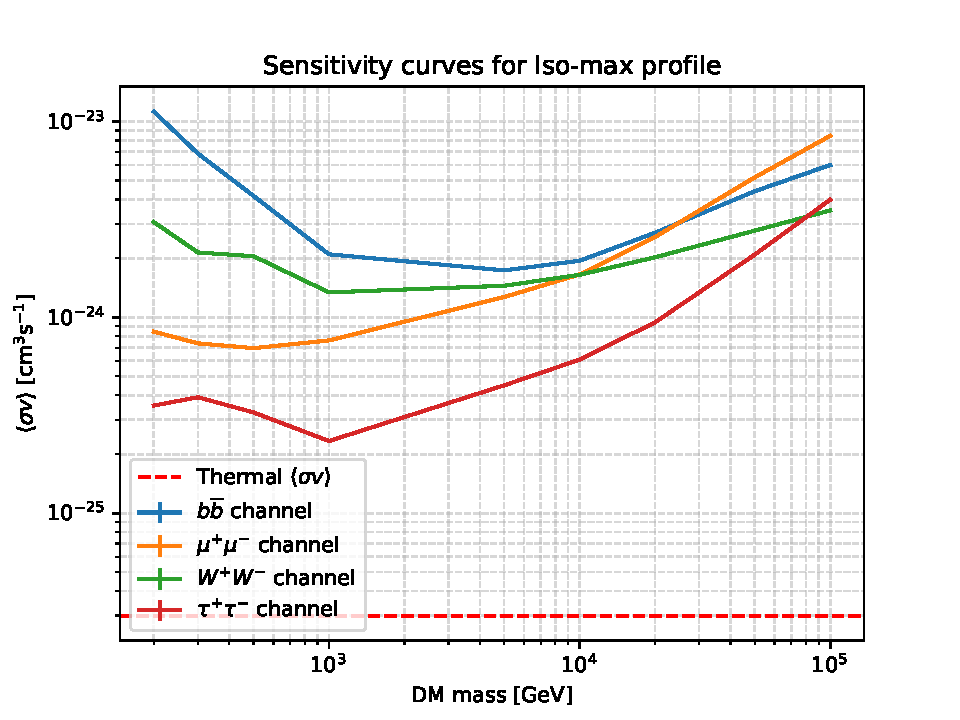
\includegraphics[width=1\textwidth]{Pictures/Limits_Iso-max.pdf}
\endminipage
  \caption{Sensitivity curves of $<\sigma v >$ vs. \gls{dm} particle mass, resulting for the profiles listed in table \ref{tab:dmprofiles}, and for four annihilation channels: $b\overline b$, $W^+W^-$, $\mu^+ \mu^-$, $\tau^+ \tau^-$.}
    \label{fig:dmsensicurves}
\end{figure}

\section{Summary and conclusions}

The deep survey of the \gls{lmc} will be an ambitious task which will account for many challenges, but that will potentially provide many scientific results and new discoveries. Besides a lot of work can be done in the subjects until \gls{cta} is fully available, in this work the first hints on the possible results of the survey have been studied.\\
Regarding the known point sources observed by other $\gamma$-ray experiments, a remarckable high significance has been obtained for all of them, meaning they will be easily detetected within the survey with a binned likelihood analysis, which will allow to characterize the sources spectra in the \gls{cta} range, at least over 100 GeV. Given the duration of the survey (>300 h), it will also be possible to study the variability of LMC-P3, for which an upper flux limit for the off-peak emission has been derived. From the artificial population of \gls{pwne} introduced in the emission model, a big number of them have been fitted with a significance sufficiently large to be detected, providing an estimation of the number of new sources that \gls{cta} will be able to detect. The computed distribution of \gls{pwne} will serve as a trace for the blind search when dealing with real data from the survey.\\
One of the most interesting aspects of the \gls{lmc} is the fact that, as an extended source, it is possible to study the structure of its $\gamma$-ray emission, allowing to probe models of \gls{cr} injection and propagation. In this work, two models of diffuse emission of \gls{cr} due to leptonic \gls{ic} scattering and hadronic interactions leading to pion decay have been tested. The possibility to take into account the structure and distribution of \gls{cr} sources in the \gls{lmc} leads to the positive result on the detection of pion-decay emission following the model described in section \ref{sec:diffusemodel}. This is however a best-case scenario, where uncertainties in the model are not taken into account. However, it is an encouraging result to make efforts on the refinement of the analysis and model computation of the diffuse emission in the \gls{lmc} for the future real data. The \gls{ic} component, on the other hand, has resulted in a too low significance, meaning it would be not possible to disentangle this emission component from the rest of the background. An upper flux limit has been derived instead for this model.\\

Finally, prospects on the detection of a possible $\gamma$-ray signal from \gls{dm} annihlation have been calculated. The results have extablished the parameter space of \gls{dm} models which will be possible to study with \gls{cta}. The main reasons to point towards the \gls{lmc} were its extended nature, which allow to rely on \gls{dm} spatial structure for its disentanglement from the background; and its realively high J-factor, comparable to other popular \gls{dm} candidates such as \gls{dsphe}. However, the big population of other $\gamma$-ray emmiters difficults the task of extracting a $\gamma$-ray signal coming from \gls{dm} annihilation. In the results presented in this thesis, several \gls{dm} profiles, annihilation channels and \gls{dm} particle masses has been tested on top of the emission model of the \gls{lmc} to compute the velocity averaged anihilation cross section needed for the model to be detected. It can be seen from picture \ref{fig:dmsensicurves}, that the majority of the models lie several orders of magnitude over the canonical thermal cross section, which is the self-annihilation cross section of \gls{wimp} \gls{dm} in the case of being a thermal relic. This result predicts that \gls{cta} will unlikely be able to exclude the canonical cross section for the typical \gls{wimp} \gls{dm} models, except for the most cuspy ones(yet not very realistic) at \gls{dm} masses $\sim 1 TeV$ (case of Gamma 1.5 profile and $\tau^+ \tau^-$ channel).\\

The work performed within the scope of this thesis will serve as a starting point for the future work that can be done regarding the \gls{lmc} \gls{ksp}. The emission model developed to perform the predictions presented will serve as a benchmark for future studies and for the analysis of real data from the \gls{lmc} survey.
Other topics wich habe been left out of the scope of this thesis, but which still will benefit from its results could be: A more detailed and realistic study on the possible new discovered sources, performing a totally blind search over the \gls{pwne} population, setting a more realistic analysis approach. The \gls{pwne} model can also be used to study the possibilities of detecting TeV haloes in the \gls{lmc}, following a similar approach as \cite{2019tevhalos}. 
Other known sources, not yet detected in the \gls{vhe} range in the \gls{lmc}, such as \gls{snr} 1987A can be studied on top of the emission model to predict its detectability within the \gls{lmc} survey.


\end{document}
 
